\documentclass [8pt] {beamer}
\usepackage[utf8]{inputenc}
\usepackage{utopia}
\usepackage{hyperref}
\usetheme{Madrid}
\usecolortheme{default}
\usepackage[T3,T1]{fontenc}
\graphicspath{ {images/} }
\newcommand{\tabitem}{~~\llap{\textbullet}~~}
\DeclareSymbolFont{tipa}{T3}{cmr}{m}{n}
\DeclareMathAccent{\invbreve}{\mathalpha}{tipa}{16}

\title[Factorización LU] {\Huge{\textbf{FACTORIZACIÓN LU \\ \ \\}}}
\subtitle {Métodos Numéricos y Estadísticos}
\author [Métodos Numéricos y Estadísticos] {Delgado Marcos, Adrián \and \\Lobato Pérez, Javier \and \\Martínez Campo, Alberto \and \\ Rodríguez Robles, Pablo \\}
\institute [] {{
\includegraphics[height=1.5cm]{ulel.png}} \\ Escuela de Ingenierías Industrial e Informática \\ Universidad de León }
\date [Ing. Aeroespacial - ULE] 

\begin{document}

\frame{\titlepage}

\AtBeginSubsection 
{ 
    \begin{frame}
        \frametitle{Índice}
        \tableofcontents[currentsection,currentsubsection]
    \end{frame}
}

\begin{frame}
    \frametitle{Factorización LU}
    \tableofcontents
\end{frame}

\section{Introducción}
    \subsection{Sistemas de ecuaciones lineales}
        \begin{frame}{Sistemas de ecuaciones lineales}
            \begin{block}{Sistemas de ecuaciones lineales}
                \Large{$\ \ \ A \cdot x = b$} \\ \ \\
                \normalsize {$\begin{array}{l}
                a_{11} x_{11} + a_{12} x_{12} + \ldots + a_{1 n} x_{1 n} = b_1\\
                a_{21} x_{21} + a_{22} x_{22} + \ldots + a_{2 n} x_{2 n} = b_2\\
                \vdots\\
                a_{n 1} x_{n 1} + a_{n 2} x_{n 2} + \ldots + a_{\tmop{nn}} x_{\tmop{nn}} = b_n
                \end{array} \left\} \rightarrow \left(\begin{array}{cccc}
                a_{11} & a_{12} & a_{13} & a_{14}\\
                a_{21} & a_{22} & a_{23} & a_{24}\\ 
                a_{31} & a_{32} & a_{33} & a_{34}\\
                a_{41} & a_{42} & a_{43} & a_{44}
                \end{array}\right) \cdot \left(\begin{array}{c}
                x_1\\ x_2\\  x_3\\  x_4
                \end{array}\right) = \left(\begin{array}{c} 
                b_1\\  b_2\\  b_3\\  b_4
                \end{array}\right)$}
            \end{block}
            \begin{block}{Operaciones elementales}
                \begin{itemize}
                    \item Intercambio de dos ecuaciones \\ $( E_i) \rightarrow ( E_j)$
                    \item Multiplicar una ecuaci{\'o}n por una constante distinta de cero \\ $( \lambda E_i) \rightarrow (E_j)$
                    \item Multiplicar a una ecuaci{\'o}n por una constante distinta de cero y sumarla a otra ecuaci{\'o}n  \\
                    $( E_i + \lambda E_j) \rightarrow ( E_j)$
                \end{itemize}
            \end{block}
        \end{frame}
        \begin{frame}{Matrices elementales}
            \begin{block}{Operaciones elementales y sus matrices}
                {Matriz identidad $\xrightarrow{\text{Operaciones elementales}}$ Matriz elemental} \\ \ \\ 
                \begin{itemize}
                    \item {$ \left( \begin{array}{ccc}
                    1 & 0 & 0 \\
                    0 & 1 & 0 \\
                    0 & 0 & 1
                    \end{array} \right )$}
                    {$\xrightarrow{E'_2 \rightarrow E_2 + 6 E_1}$}
                    {$\left( \begin{array}{ccc}
                    1 & 0 & 0\\
                    6 & 1 & 0\\
                    0 & 0 & 1
                    \end{array} \right)$}
                    \item{$\left( \begin{array}{cccc}
                    1 & 0 & 0 & 0\\
                    0 & 1 & 0 & 0\\
                    0 & 0 & 1 & 0\\     
                    0 & 0 & 0 & 1
                    \end{array} \right)$}
                    {$\xrightarrow{E'_3 \rightarrow E_3 - 5 E_1}$}
                    {$\left( \begin{array}{cccc}
                    1 & 0 & 0 & 0\\
                    0 & 1 & 0 & 0\\
                    - 5 & 0 & 1 & 0\\
                    0 & 0 & 0 & 1
                    \end{array} \right)$}  \\ \ \\ \ \\
                \end{itemize}
                {$E'_2 \rightarrow E_2 - 3 E_1 \Rightarrow \left( \begin{array}{ccc}
                1 & 0 & 0\\
                - 3 & 1 & 0\\
                0 & 0 & 1
                \end{array} \right) \left( \begin{array}{ccc}
                6 & - 1 & 1\\
                7 & 2 & 3\\
                0 & - 3 & - 2
                \end{array} \right) = \left( \begin{array}{ccc}
                6 & - 1 & 2\\
                - 11 & 5 & - 3\\
                0 & - 3 & - 2
                \end{array} \right)$} \\ \ \\ \ \\
                {$E \cdot E^{- 1} = \tmop{Id}  \Rightarrow  \ \ \ \ \ \ E = \left( \begin{array}{ccc}
                1 & - 2 & 0\\
                0 & 1 & 0\\
                0 & 0 & 1
                \end{array} \right) \ \ \ \ \ \ \ \ E^{- 1} =
                \left( \begin{array}{ccc}
                1 & 2 & 0\\
                0 & 1 & 0\\
                0 & 0 & 1
                \end{array} \right)$}
            \end{block}
        \end{frame}
        \begin{frame}{Métodos de resolución de sistemas de ecuaciones lineales}
            \begin{block}{Métodos directos}
                \begin{tabular}{ll} 
                    \tabitem Eliminaci{\'o}n gaussiana & $\tmop{Ax} = b \rightarrow \tmop{Ux} = c$\\ 
                    \tabitem Descomposici{\'o}n LU & $\tmop{Ax} = b \rightarrow \tmop{LUx} = b$\\ 
                    \tabitem Eliminaci{\'o}n Gauss-Jordan & $\tmop{Ax} = b \rightarrow \tmop{Ix} = c$ \\ 
                \end{tabular}
            \end{block}
            \begin{block} {Métodos iterativos}
                \begin{tabular}{l}
                    \tabitem {Método de Jacobi} \\
                    \tabitem {Método de Gauss-Seidel} \\ 
                    \tabitem {Método de relajación (SOR)} \\
                \end{tabular}
            \end{block}
        \end{frame}
        \begin{frame}{Eliminación gaussiana}
            \begin{block}{Fase de eliminación}
                {$E_i \rightarrow E_i - \lambda \cdot E_j \ \ \ \ \ \ \ ( multiplicador: 
                \lambda = \dfrac{a_{i j}}{a_{i i}})$} \\ \ \\
                \begin{center}
                    {$\left( \begin{array}{ccc}
                    u_{11} & u_{12} & u_{13}\\ 0 & u_{22} & u_{23}\\ 0 & 0 & u_{33}
                    \end{array} \right) \cdot \left( \begin{array}{c}
                    x_1\\  x_2\\  x_3
                        \end{array} \right) = \left( \begin{array}{c}
                    c_1\\  c_2\\  c_3
                    \end{array} \right)$}
                \end{center}
            \end{block}
            \begin{block}{Sustitución regresiva}
                $ x_n = \dfrac{1}{u_{\tmop{nn}}} c_{n}\\ \ \\$
                $x_i = \dfrac{1}{u_{\tmop{ii}}} \left( c_i - 
                \displaystyle\sum^n_{j = i + 1} u_{\tmop{ij}}
                x_j \right) \rightarrow i = n - 1 , \ldot , 1$
            \end{block}
        \end{frame}
        \begin{frame}{Ejemplo de eliminación gaussiana}
            \begin{exampleblock}{Fase de eliminación:}
                {$\left( \[\arraycolsep=3pt\def\arraystretch{1} \begin{array}{ccc}
                4 & - 2 & 1\\
                - 2 & 4 & - 2\\
                1 & - 2 & 4
                \end{array} \right) \left( \[\arraycolsep=1pt\def\arraystretch{1} \begin{array}{c}
                x_1\\  x_2\\  x_3
                \end{array} \right) = \left( \[\arraycolsep=1pt\def\arraystretch{1} \begin{array}{c}
                11\\  - 16\\  17
                \end{array} \right) \xrightarrow{E'_2 \rightarrow E_2 - \frac{- 2}{4} E_1}
                \left( \[\arraycolsep=3pt\def\arraystretch{1} \begin{array}{ccc}
                4 & - 2 & 1\\
                0 & 3 & - 1.5\\
                1 & - 2 & 4
                \end{array} \right) \left( \[\arraycolsep=1pt\def\arraystretch{1} \begin{array}{c}
                x_1\\  x_2\\  x_3
                \end{array} \right) = \left( \[\arraycolsep=1pt\def\arraystretch{1} \begin{array}{c}    
                11\\  - 10.5\\  17
                \end{array} \right) \\ \ \\ \ \\ \left( \[\arraycolsep=3pt\def\arraystretch{1} \begin{array}{ccc}
                4 & - 2 & 1\\
                0 & 3 & - 1.5\\
                1 & - 2 & 4
                \end{array} \right) \left( \[\arraycolsep=1pt\def\arraystretch{1} \begin{array}{c}
                x_1\\  x_2\\  x_3
                \end{array} \right) = \left( \[\arraycolsep=1pt\def\arraystretch{1} \begin{array}{c}
                11\\  - 10.5\\  17  
                \end{array} \right) \xrightarrow{E'_3 \rightarrow E_3 - \frac{1}{4} E_1}     
                \left( \[\arraycolsep=3pt\def\arraystretch{1} \begin{array}{ccc}
                4 & - 2 & 1\\
                0 & 3 & - 1.5\\
                0 & - 1.5 & 3.75
                \end{array} \right) \left( \[\arraycolsep=1pt\def\arraystretch{1} \begin{array}{c}
                x_1\\  x_2\\  x_3
                \end{array} \right) = \left( \[\arraycolsep=1pt\def\arraystretch{1} \begin{array}{c}
                11\\  - 10.5\\  14.25 
                \end{array} \right) \\ \ \\ \ \\ \left( \[\arraycolsep=2.5pt\def\arraystretch{1} \begin{array}{ccc}
                4 & - 2 & 1\\
                0 & 3 & - 1.5\\
                0 & - 1.5 & 3.75
                \end{array} \right) \left( \[\arraycolsep=1pt\def\arraystretch{1} \begin{array}{c}
                x_1\\  x_2\\  x_3
                \end{array} \right) = \left( \[\arraycolsep=0.5pt\def\arraystretch{1} \begin{array}{c}
                11\\  - 10.5\\  14.25 
                \end{array} \right) \xrightarrow{E'_3 \rightarrow E_3 - \frac{- 1.5}{3} E_2}
                \left( \[\arraycolsep=2.5pt\def\arraystretch{1} \begin{array}{ccc}
                4 & - 2 & 1\\
                0 & 3 & - 1.5\\
                0 & 0 & 3
                \end{array} \right) \left( \[\arraycolsep=1pt\def\arraystretch{1} \begin{array}{c}
                x_1\\  x_2\\  x_3
                \end{array} \right) = \left( \[\arraycolsep=1pt\def\arraystretch{1} \begin{array}{c}        
                11\\  - 10.5\\  9
                \end{array} \right)$ \\ \ \\ \ \\ }
                \begin{figure}
                    \centering
                    {$\left\{ \begin{array}{ccccc}
                    4 x_1 & - 2 x_2 & + x_3 & = & 11\\
                    & 3 x_2 & - 1.5 x_3 & = & - 10.5\\
                    &  & 3 x_3 & = & 9
                    \end{array} \right\}$}
                \end{figure} \\ \ \\ 
            \end{exampleblock}
        \end{frame}
        \begin{frame}{Ejemplo de eliminación gaussiana}
            \begin{exampleblock}{Sustitución regresiva}
                {$\ \ \ \begin{array}{rl}
                \left. \[\arraycolsep=2pt\def\arraystretch{1} \begin{array}{ccccc}
                4 x_1 & - 2 x_2 & + x_3 & = & 11\\
                & 3 x_2 & - 1.5 x_3 & = & - 10.5\\  
                &  & 3 x_3 & = & 9
                \end{array} \right\} & \rightarrow x_3 = \dfrac{1}{3} \cdot 9 = 3\\ \ \\
                \left. \[\arraycolsep=2pt\def\arraystretch{1} \begin{array}{ccccc}
                4 x_1 & - 2 x_2 & + x_3 & = & 11\\
                & 3 x_2 & - 1.5 x_3 & = & - 10.5\\
                &  & x_3 & = & 3
                \end{array} \right\} & \rightarrow x_2 = \dfrac{1}{3} \cdot ( - 10.5 + 1.5 \cdot 3) = - 2\\ \ \\ 
                \left. \[\arraycolsep=3pt\def\arraystretch{1} \begin{array}{ccccc}
                4 x_1 & - 2 x_2 & + x_3 & = & 11\\
                &  & x_2 & = & - 2\\
                &  & x_3 & = & 3
                \end{array} \right\} & \rightarrow x_1 = \dfrac{1}{4} \cdot ( 11 - 1 \cdot 3 + 2 \cdot ( - 2)) = 1\\ \ \\
                \left\{ \[\arraycolsep=3pt\def\arraystretch{1} \begin{array}{ccc}
                x_1 & = & 1\\
                x_2 & = & - 2\\
                x_3 & = & 3
                \end{array} \right\} & \ \end{array}$}
            \end{exampleblock}
        \end{frame}
        \begin{frame}{Elimación de Gauss-Jordan}
                \begin{block} {Eliminación de Gauss-Jordan}
                { $ \[ \left(  \[\arraycolsep=2pt\def\arraystretch{1} \begin{array}{lll}
                a_{11} & a_{12} & a_{13}\\
                a_{21} & a_{22} & a_{23}\\
                a_{31} & a_{32} & a_{33}
                \end{array} \left| \begin{array}{l}
                b_1\\ b_2\\ b_3 
                \end{array} \right. \right) \rightarrow \left(  \[\arraycolsep=2pt\def\arraystretch{1} \begin{array}{ccc}
                l_{11} & l_{12} & l_{13}\\
                0 & l_{22} & l_{23}\\
                0 & 0 & l_{33}
               \end{array} \left| \begin{array}{l}
                b'_1\\ b'_2\\ b'_3
               \end{array} \right. \right) \rightarrow \left(  \[\arraycolsep=2pt\def\arraystretch{1} \begin{array}{ccc}
                d_{11} & 0 & 0\\
                0 & d_{22} & 0\\
                0 & 0 & d_{33}
               \end{array} \left| \begin{array}{l}
                b''_1\\ b''_2\\ b''_3       
                \end{array} \right. \right) \rightarrow \left(  \[\arraycolsep=2.5pt\def\arraystretch{1}
                \begin{array}{ccc}
                1 & 0 & 0\\
                0 & 1 & 0\\
                0 & 0 & 1
               \end{array} \left| \begin{array}{l}
                c_1\\ c_2\\ c_3
               \end{array} \right. \right)$}
            \end{block}
            \begin{block}{Uso en el cálculo de inversas}
                \begin{center}
                    {$\left. \left( \begin{array}{ccc} & & \\ & A & \\ & & \\ 
                    \end{array} \right| \begin{array}{lll}
                    1 & 0 & 0\\
                    0 & 1 & 0\\
                    0 & 0 & 1
                    \end{array} \right) \rightarrow \left( \begin{array}{lll}
                    1 & 0 & 0\\
                    0 & 1 & 0\\
                    0 & 0 & 1
                    \end{array} \left| \begin{array}{ccc} & & \\ & A^{- 1} & \\ & & \\ \end{array} \right. \right)$}
                \end{center}
            \end{block}
        \end{frame}
        \begin{frame}{Ejemplo de Gauss-Jordan}
            \begin{exampleblock}{Ejemplo:}
                {$\left\{ \begin{array}{r}
                x + y + z = 5\\
                2 x + 3 y + 5 z = 8\\
                4 x + 5 z = 2
                \end{array} \right\} \xrightarrow{forma \ \ matricial} \left(
                \begin{array}{lll}
                1 & 1 & 1\\
                2 & 3 & 5\\
                4 & 0 & 5
                \end{array} \left| \begin{array}{l}
                5\\  8\\  2
                \end{array} \right. \right) \\ \ \\ 
                \[\arraycolsep=3pt\def\arraystretch{1} \left( \begin{array}{ccc}
                1 & 1 & 1\\
                2 & 3 & 5\\
                4 & 0 & 5
                \end{array} \left| \begin{array}{c}
                5\\     8\\     2
                \end{array} \right. \right) \underset{E'_3 = E_3 - 4 E_1}{\xrightarrow{E'_2 = E_2 - 2 E_1}} \left( 
                \[\arraycolsep=3pt\def\arraystretch{1} \begin{array}{ccc}
                1 & 1 & 1\\
                0 & 1 & 3\\
                0 & - 4 & 1
                \end{array} \left| \begin{array}{c}
                5\\ - 2\\ - 18
                \end{array} \right. \right) \xrightarrow{E'_3 = E_3 + 4 E_2} \left(
                \[\arraycolsep=3pt\def\arraystretch{1}
                \begin{array}{ccc}
                1 & 1 & 1\\
                0 & 1 & 3\\ 
                0 & 0 & 13
                \end{array} \left| \begin{array}{c}
                5\\ - 2\\ - 26
                \end{array} \right. \right) \xrightarrow{E'_3 = \frac{E_3}{13}} \]$} \\ \ \\
                {$\rightarrow \left( \[\arraycolsep=3pt\def\arraystretch{1} \begin{array}{ccc}
                1 & 1 & 1\\
                0 & 1 & 3\\
                0 & 0 & 1
                \end{array} \left| \begin{array}{c}
                5\\  - 2\\  - 2
                \end{array} \right. \right) \underset{E'_1 = E_1 - 3 E_3}{\xrightarrow{E'_2 =
                E_2 - 3 E_3}} \left( \begin{array}{ccc}
                1 & 1 & 0\\
                0 & 1 & 0\\
                0 & 0 & 1
                \end{array} \left| \begin{array}{c}
                7\\  4\\  - 2
                \end{array} \right. \right) \underset{}{\xrightarrow{E'_1 = E_1 - E_2}} \left(
                \begin{array}{ccc}
                1 & 0 & 0\\
                0 & 1 & 0\\
                0 & 0 & 1
                \end{array} \left| \begin{array}{c}
                3\\  4\\  - 2
                \end{array} \right. \right)$} \\ \ \\ \ \\ 
                {SOLUCIÓN: $\left\{ \begin{array}{c}
                x = 3\\  y = 4\\  z = - 2
                \end{array} \right\}$}
            \end{exampleblock}
        \end{frame}
        \begin{frame}{Sustitución progresiva}
            \begin{block} {Algoritmo de la sustitución progresiva}
                $x_1 = \dfrac{1}{u_{11}} b_{1}\\ \ $ \\ \ \\
                $ x_i = \dfrac{1}{u_{\tmop{ii}}} \left( b_i - \displaystyle\sum^n_{j = 1} u_{\tmop{ij}} x_j \right) 
                \rightarrow i = 2 , 3, \ldots, n $
            \end{block}
            \begin{exampleblock} {Ejemplo de sustitución progresiva:}
                {$\begin{array}{rl}
                \left. \[\arraycolsep=1.2pt\def\arraystretch{1} \begin{array}{ccccc}
                3 x_1 &  &  & = & 9\\
                - 1.5 x_1 & 3 x_2 &  & = & - 10.5\\
                x_1 & - 2 x_2 & + 4 x_3 & = & 11
                \end{array} \right\} & \nocomma x_1 = \dfrac{1}{3} \cdot 9 = 3\\
                \left. \[\arraycolsep=1.2pt\def\arraystretch{1} \begin{array}{ccccc}
                x_1 &  &  & = & 3\\
                - 1.5 x_1 & 3 x_2 &  & = & - 10.5\\
                x_1 & - 2 x_2 & + 4 x_3 & = & 11
                \end{array} \right\} & x_2 = \dfrac{1}{3} \cdot ( - 10.5 + 1.5 \cdot 3) = -2\\
                \left. \[\arraycolsep=1.2pt\def\arraystretch{1} \begin{array}{ccccc}
                x_1 &  &  & = & 3\\
                & x_2 &  & = & - 2\\
                x_1 & - 2 x_2 & + 4 x_3 & = & 11
                \end{array} \right\} & x_3 = \dfrac{1}{4} \cdot ( 11 - 1 \cdot 3 + 2 \cdot ( - 2)) = 1\\
                \end{array} \\ \ \\  $}
                \ \ \ \ \ \ \ \ \ \  \ \ \ \ \ \ \ \ \ \ \ \ \  \ \ \  SOLUCI{\'O}N: { 
                $\left\{ \begin{array}{ccc}
                x_1 & = & 3\\
                x_2 & = & - 2\\
                x_3 & = & 1
                \end{array} \right\} $}
            \end{exampleblock}
        \end{frame}
    \subsection{Pivoteo}
        \begin{frame} {Importancia de tener un buen pivote}
            \begin{exampleblock} {Ejemplo:} 
                {Resolución del sistema S por Gauss (con mal pivote):} \\
                S = $\left \{ \begin{array}{l}
                0.003 x_1 + 59.14 x_2 = 59.17\\
                5.291 x_1 - 6.130 x_2 = 46.78
                \end{array} \right \} $ \\ \ \\ 
                \begin{itemize}
                    \item {Redondeando a 4 cifras:} \\
                    $\left \{  \[\arraycolsep=3pt\def\arraystretch{1} \begin{array}{l}
                    0.003 x_1 + 59.14 x_2 = 59.17\\
                    5.291 x_1 - 6.130 x_2 = 46.78
                    \end{array} \right \} 
                    \xrightarrow [m_{21}=\frac{a_{2 1}}{a_{1 1}} = \frac {5.291}{0.003} = 1764] {E_2' = E_2 -  m_{21} \cdot E_1}  
                    \left \{  \[\arraycolsep=3pt\def\arraystretch{1} \begin{array}{l}
                    0.003 x_1 + 59.14 x_2 \approx 59.17\\
                    -104300 x_2 \approx -104400
                    \end{array} \right \}
                    \rightarrow \\ \ \ \ \rightarrow 
                    \left \{ \begin{array}{l}
                    x_1 \approx - 10\\
                    x_2 \approx 1.001
                    \end{array} \right \} $
                \end{itemize}
                \begin{itemize}
                    \item{Sin redondear:} \\
                    $\left \{ \begin{array}{l}
                    0.003 x_1 + 59.14 x_2 = 59.17\\
                    5.291 x_1 - 6.130 x_2 = 46.78
                    \end{array} \right \} 
                    \xrightarrow [m_{21}= 1763. \invbreve{6}] {E_2' = E_2 - m_{21} \cdot E_1}  
                    \left \{ \begin{array}{l}
                    0.003 x_1 + 59.14 x_2 = 59.17\\
                    -104309.37 \invbreve{6} x_2 = -104309.37 \invbreve{6}
                    \end{array} \right \}
                    \rightarrow \\ \ \ \ \rightarrow 
                    \left \{ \begin{array}{l}
                    x_1 = 10\\
                    x_2 = 1
                    \end{array} \right \} $
                \end{itemize}
            \end{exampleblock}
        \end{frame}
        \begin{frame} {Pivoteo parcial}
            \begin{block}{Pivoteo parcial}
                {$a_{_{p j}} = \underset{i = j, \ldots, n}{\max}  \{ | a_{i j} | \} \rightarrow
                \tmop{intercambio} \tmop{filas} E_p \leftrightharpoons E_i $}
            \end{block}
            \begin{exampleblock}{Ejemplo de pivoteo parcial:}
                {S = $\left \{ \begin{array}{l}
                0.003 x_1 + 59.14 x_2 = 59.17\\
                5.291 x_1 - 6.130 x_2 = 46.78
                \end{array} \right \} $ \\ \ \\ \ \\}
                {$a_{_{p j}} = \max \{ | a_{11} |, | a_{21} | \} = \max \{ | 0.003 |, | 5.291 | \} = | 5.291 | = | a_{21} |} \\ 
                {\[ \left\{ \[\arraycolsep=3pt\def\arraystretch{1}  \begin{array}{l}
                5.291 x_1 - 6.130 x_2 = 46.78\\ 
                0.003 x_1 + 59.14 x_2 = 59.17
                \end{array} \right\} 
                \xrightarrow[m_{21} = \frac{a_{21}}{a_{11}} = \frac{0.003}{5.291} = 0.000567]{E_2' = E_2 - m_{21}
                E_1} \left\{ \begin{array}{l}
                5.291 x_1 - 6.130 x_2 = 46.78\\
                59.14 x_2 = 59.14
                \end{array} \right\} \rightarrow  \\ \rightarrow \left\{ \begin{array}{l}
                x_1 = 10\\
                x_2 = 1
                \end{array} \right\} \]$}
            \end{exampleblock}
        \end{frame}
        \begin{frame} {Pivoteo parcial}
            \begin{block}{Matriz de permutación}
               {Para hacer un cambio de filas, se emplea una matriz $P_n$ (matriz identidad modificada) para que al multiplicarla por la izquierda los cambios afecten a las filas :}
                $ \left \begin{array}{l}
                I d_2 = \left( \begin{array}{cc}
                1 & 0\\
                0 & 1
                \end{array} \right) \\
                S = \left( \begin{array}{cc}
                0.003 & 59.14\\
                5.291 & - 6.130
                \end{array} \right)
                \end{array} \right\} \xrightarrow{E^{ ({Id})}_1 \leftrightharpoons E^{({Id})}_2} P = \left( \begin{array}{ll}
                0 & 1\\
                1 & 0
                \end{array} \right) \rightarrow P \cdot S = \left( \begin{array}{cc}
                5.291 & - 6.130\\
                0.003 & 59.14
                \end{array} \right) $ \\ \ \\ 
                {Una buena matriz $P$ cumple $P^{- 1} = P^t$ \\}
            \end{block}
            \begin{alertblock}{Fallo del pivoteo parcial}
                {Vamos a multiplicar ahora $E_1$ por $10^4$ y a resolver el sistema obtenido.} \\ \ \\
                $\left\{ \begin{array}{l}
                30.00 x_1 + 591400 x_2 = 591700\\
                5.291 x_1 - 6.130 x_2 = 46.78
                \end{array} \right\} \xrightarrow[m_{21} = \frac{5.291}{30.00} = 0.1764]{E_2' = E_2 - m_{21} \cdot E_1} \left\{ 
                \begin{array}{l}
                30.00 x_1 + 591400 x_2 = 591700\\
                - 104300 x_2 = - 104400
                \end{array} \right\} \rightarrow \left\{ \begin{array}{l}
                x_1 = - 10\\
                x_2 = 1.001
                \end{array} \right\}$ \\ \ \\
                {Volvemos a obtener resultados incorrectos por tener un mal pivote, ya que $a_{11}$ es muy grande respecto $a_{21}$.}
            \end{alertblock}
        \end{frame}
        \begin{frame} {Pivoteo parcial escalado}
            \begin{block} {Elección de pivote} 
            \begin{columns}
                \column{0.62\textwidth}
                    \begin{itemize}
                        \item  {$S_i = \underset{j = 1, \ldots, n}{\max}  \{ | a_{i j} | \} $ \\ \ \\}
                        \item { $\dfrac{| a_{p 1} |}{S_p} = \underset{k = 1, \ldots, n}{\max} \dfrac{| a_{k 1} |}{S_k} 
                        \ \ (p = $ {nueva fila pivote} ) \\}
                        \item {$\tmop{intercambio \ } E_p \leftrightharpoons E_k$}
                    \end{itemize}
                \column{0.38\textwidth}
                    $\left( \begin{array}{lllll}
                    a_{11} & a_{12} & a_{13} & \ldots & a_{1 n}\\
                    a_{21} & a_{22} & a_{23} & \ldots & a_{2 n}\\
                    a_{31} & a_{32} & a_{33} & \ldots & a_{3 n}\\
                    \vdots & \vdots & \vdots & \ddots & \vdots\\
                    a_{n 1} & a_{2 n} & a_{3 n} & \ldots & a_{n n}
                    \end{array} \right)$
            \end{columns}
        \end{block}
            \begin{exampleblock}{Ejemplo:}
                \begin{columns}
                    \column{0.55\textwidth}
                        \large{
                        $\dfrac{| a_{11} |}{S_1} = \frac{30.00}{\max \{ | 30.00 |, | 591400 | \}} = 0.5073 \times 10^{- 4} $\\  \ \\ 
                        $\ \dfrac{| a_{21} |}{S_2} = \frac{5.291}{\max \{ | 5.291 |, | 6.130 | \}} = 0.8631$}
                    \column{0.425\textwidth}
                        S = $\left \{  \[\arraycolsep=1pt\def\arraystretch{1}\begin{array}{l}
                        30.00 x_1 + 591400 x_2 = 591700\\
                        5.291 x_1 - 6.130 x_2 = 46.78
                        \end{array} \right \} $
                \end{columns}
                \\ \ \\ \ \\ \ {$\tmop{Intercambio \ }E_1 \leftrightharpoons E_2$} \\ 
                $\left\{ \begin{array}{l}
                5.291 x_1 - 6.130 x_2 = 46.78\\
                30.00 x_1 + 591400 x_2 = 591700
                \end{array} \right\} \xrightarrow[m_{21} =\frac{30.00}{5.291} = 5.670]{E_2' = E_2 - m_{21} \cdot E_1}
                \left\{ \begin{array}{l}
                5.291 x_1 - 6.130 x_2 = 46.78\\
                591434.76 x_2 = 591434.76
                \end{array} \right\} \rightarrow \left\{ \begin{array}{l}
                x_1 = 10\\
                x_2 = 1
                \end{array} \right\}$
            \end{exampleblock}
        \end{frame}
%-------------------------------------------------------------------------
\section{Factorización LU}
    \subsection{Factorización LU}
        \begin{frame}{Factorización LU}
            \begin{block}{Descomposición de A}
                {\Large{\ \ \ $A = L \cdot U $}}
            \end{block}
            \begin{block}{Algoritmo de resolución}
                \ \ \ \large{$A \cdot X = b \xrightarrow{A = L \cdot U} L \cdot U \cdot X = b \rightarrow \left\{ \begin{array}{l}
                \begin{array}{l}
                L \cdot Y = b\\
                U \cdot X = Y
                \end{array}
                \end{array} \right\}$ \\ \ \\ \ \\ }
                {$ \left( \begin{array}{ll}
                A_{11} & A_{12}\\   
                A_{21} & A_{22}
                \end{array} \right) \cdot
                \left( \begin{array}{l}
                x_1\\ x_2
                \end{array} \right) = 
                \left( \begin{array}{l}
                b_1\\
                b_2
                \end{array} \right) $} \\ \ \\ \ \\ 
                {$ \left( \begin{array}{cc}
                L_{11} & 0\\
                L_{12} & L_{22}
                \end{array} \right) \cdot \left( \begin{array}{cc}
                U_{11} & U_{12}\\
                0 & U_{22}
                \end{array} \right) \cdot \left( \begin{array}{l}
                x_1\\ x_2
                \end{array} \right) = \left( \begin{array}{l}
                b_1\\ b_2
                \end{array} \right) $ } \\ \ \\ \ \\
                {$ \underbrace{\left( \begin{array}{cc}
                L_{11} & 0\\
                L_{12} & L_{22}
                \end{array} \right) \cdot 
                \overbrace{\left( \begin{array}{l}
                y_1\\ y_2
                \end{array} \right )}^{U \cdot X = Y} = 
                \left( \begin{array}{l}
                b_1\\ b_2
                \end{array} \right)}_{L \cdot Y = b} $ } \ \ \ \ \ \ \
                {$ \underbrace{ \left( \begin{array}{cc}
                U_{11} & U_{12}\\
                0 & U_{22}
                \end{array} \right) \cdot 
                \left( \begin{array}{l}
                x_1\\ x_2
                \end{array} \right) = 
                \left( \begin{array}{l}
                y_1\\ y_2
                \end{array} \right )}_ {U \cdot X = Y}$ }
            \end{block}
        \end{frame}
        \begin{frame}{Factorización LU}
            \begin{block}{Algoritmo de resolución (y II)}
                {$ L\cdot Y = b \rightarrow \left\{ \begin{array}{l}
                L_{11} y_1 = b_1  \\
                L_{12} y_1 + L_{22} y_2 = b_2
                \end{array} \right\} \rightarrow \left[ \begin{array}{l}
                y_1 = \dfrac{1}{L_{11}} b_1 \\ \ \\
                y_2 = \dfrac{1}{L_{22}} \left( b_2 - L_{12} y_1 \right) 
                \end{array} \right] $} \\ \ \\
                \begin{itemize}
                    \item  {$y_i = \dfrac{1}{L_{i i}}  \left( b_i - \displaystyle\sum_{j = 1}^{i - 1} L_{i j} y_j
                    \right) \rightarrow \tmop{siendo \ } i = 2, \ldots, n$ \\ \ \\ \ \\ }
                \end{itemize}
                {$ U\cdot X = Y \rightarrow \left\{ \begin{array}{l}
                U_{11} x_1 + U_{12} x_2 = y_1 \\
                U_{22} x_2 = y_2
                \end{array} \right\} \rightarrow
                \left[ \begin{array}{l}
                x_2 = \dfrac{1}{U_{22}} y_2 \\ \ \\
                x_1 = \dfrac{1}{U_{11}} \left( y_1 - U_{12} x_2 \right) 
                \end{array} \right]
                \rightarrow x_n = \dfrac{1}{U_{i i}} y_n$}\\ \ \\
                \begin{itemize}
                    \item {$x_n = \dfrac{1}{U_{i i}}  \left( y_i - \displaystyle\sum_{j = i + 1}^n U_{i j} x_j \right)
                    \rightarrow \tmop{siendo \ } i = n - 1, \ldots, 1$}
                \end{itemize}
            \end{block}
        \end{frame}
        \begin{frame}{Obtención de matrices L y U}
            \begin{exampleblock}{Ejemplo de obtención de matrices L y U:}
                {$A = \left( \begin{array}{ccc}
                -2 & 5 & 2\\ 
                1 & 3 & -6\\   
                4 & 6 & 9
                \end{array} \right)\ \ \ \ \ \ B = \left( \begin{array}{c}
                b 1\\  b 2\\  b 3
                \end{array} \right)  \ \ \ \ \ \
                X = \left( \begin{array}{c} 
                x_1\\x_2\\ x_3
                \end{array} \right) $ \\ \ \\ \rule{121mm}{0.1mm} \\ \ \\}
               {$U_{\tmop{inicial}} = \left( \[\arraycolsep=3pt\def\arraystretch{1} \begin{array}{ccc}
                - 2 & 5 & 2\\
                1 & - 3 & 5\\
                4 & 1 & 2   
                \end{array} \right) \xrightarrow{F'_2 \rightarrow F_1 + 2 F_2} \left( \[\arraycolsep=3pt\def\arraystretch{1}
                \begin{array}{ccc}
                - 2 & 5 & 2\\
                0 & - 1 & 12\\
                4 & 1 & 3
                \end{array} \right)  \xrightarrow{F'_3 \rightarrow F_3 + 2 F_1} \left( \[\arraycolsep=3pt\def\arraystretch{1}
                \begin{array}{ccc}
                - 2 & 5 & 2\\
                0 & - 1 & 12\\  
                0 & 11 & 6
                \end{array} \right) \rightarrow \ \\ \ \\
                \xrightarrow{F'_3 \rightarrow 11 F_2 + F_3} \left( \[\arraycolsep=3pt\def\arraystretch{1}
                \begin{array}{ccc}
                - 2 & 4 & 9\\
                0 & - 1 & 12\\
                0 & 0 & 22
                \end{array} \right)$} \\ \ \\ \ \\ \ \\
                {$L_{\tmop{inicial}} = \left( \begin{array}{ccc}
                1 & 0 & 0\\
                0 & 1 & 0\\
                0 & 0 & 1
                \end{array} \right) \xrightarrow{\tmop{Factor} \ 1} \left( \begin{array}{ccc}
                1 & 0 & 0\\
                - 2 & 1 & 0\\
                0 & 0 & 1
                \end{array} \right) \xrightarrow{\tmop{Factor} \ 2} \left( \begin{array}{ccc}
                1 & 0 & 0\\
                - 2 & 1 & 0\\
                - 2 & 0 & 1
                \end{array} \right) \rightarrow \\ \ \\ \xrightarrow{\tmop{Factor} \ 3} \left( \begin{array}{ccc}
                1 & 0 & 0\\
                - 2 & 1 & 0\\
                - 2 & - 11 & 1      
                \end{array} \right)$}
            \end{exampleblock}
        \end{frame}
        \begin{frame}{Descomposiciones}
            \begin{block}{Tipos de descomposiciones}
                \begin{tabular}{ll} 
                    \tabitem Descomposici{\'o}n de Doolitle & $ L_{ii}=1 \rightarrow i = 1,2,\ldots, n $\\ 
                    \tabitem Descomposici{\'o}n de Court & $ U_{ii}=1 \rightarrow i = 1,2,\ldots, n $\\ 
                    \tabitem Descomposici{\'o}n de Choleski & $ L = U ^ T$ \\ 
                \end{tabular} \\ \ \\ \ \\
                \begin{center}
                    {$\left\{ \begin{array}{lll}
                    l_{11} \cdot u_{11} & = & a_{11}\\      
                    l_{11} \cdot u_{12} & = & a_{12}\\
                    l_{11} \cdot u_{13} & = & a_{13}\\
                    l_{21} \cdot u_{11} & = & a_{21}\\
                    l_{21} \cdot u_{12} + l_{22} \cdot u_{22} & = & a_{22}\\
                    l_{21} \cdot u_{13} + l_{22} \cdot u_{23} & = & a_{23}\\
                    l_{31} \cdot u_{11} & = & a_{31}\\
                    l_{31} \cdot u_{12} + l_{32} \cdot u_{22} & = & a_{32}\\
                    l_{31} \cdot u_{13} + l_{32} \cdot u_{23} + l_{33} \cdot u_{33} & = & a_{33}
                    \end{array} \right\}$} \\ \ \\ \ \\ \ \\
                    {$\left( \begin{array}{ccc}
                    l_{11} & 0 & 0\\
                    l_{21} & l_{22} & 0\\
                    l_{31} & l_{32} & l_{33}
                    \end{array} \right) \cdot \left( \begin{array}{ccc}
                    u_{11} & u_{12} & u_{13}\\
                    0 & u_{22} & u_{23}\\
                    0 & 0 & u_{33}
                    \end{array} \right) = \left( \begin{array}{ccc}
                    a_{11} & a_{12} & a_{13}\\
                    a_{21} & a_{22} & a_{23}\\
                    a_{31} & a_{32} & a_{33}
                    \end{array} \right)$}
                \end{center}
            \end{block}
        \end{frame}
    \subsection{Factorización en términos de operaciones elementales}
        \begin{frame}{Un primer algoritmo}
            \begin{exampleblock} {Ejemplo:}
                {$A = \left( \begin{array}{ccc}
                - 4 & - 3 & 1\\
                8 & 11 & - 1\\
                4 & 18 & 5
                \end{array} \right)$} 
                {$\Rightarrow L \cdot U = \left( \begin{array}{ccc}
                1 & 0 & 0\\
                0 & 1 & 0\\
                0 & 0 & 1
                \end{array} \right) \left( \begin{array}{ccc}
                - 4 & - 3 & 1\\
                8 & 11 & - 1\\
                4 & 18 & 5
                \end{array} \right)$} \\ \ \\ \ \\ \ \\
                {$E'_2 = E_2 + 2 E_1 \Rightarrow E = \left( \begin{array}{ccc} 
                1 & 0 & 0\\
                2 & 1 & 0\\
                0 & 0 & 1
                \end{array} \right) \Rightarrow $} 
                {$A =LE^{- 1}EU$} \\ \ \\ \ \\ 
                {$A = \left( \[\arraycolsep=2pt\def\arraystretch{1} \begin{array}{ccc}
                1 & 0 & 0\\
                0 & 1 & 0\\
                0 & 0 & 1
                \end{array} \right) \left( \[\arraycolsep=3pt\def\arraystretch{1} \begin{array}{ccc}
                1 & 0 & 0\\
                - 2 & 1 & 0\\   
                0 & 0 & 1
                \end{array} \right) \left( \[\arraycolsep=2pt\def\arraystretch{1} \begin{array}{ccc}
                1 & 0 & 0\\
                2 & 1 & 0\\
                0 & 0 & 1
                \end{array} \right) \left( \[\arraycolsep=3pt\def\arraystretch{1} \begin{array}{ccc}
                - 4 & - 3 & 1\\
                8 & 11 & - 1\\
                4 & 18 & 5
                \end{array} \right) = \left( \[\arraycolsep=3pt\def\arraystretch{1} \begin{array}{ccc}
                1 & 0 & 0\\
                - 2 & 1 & 0\\
                0 & 0 & 1
                \end{array} \right)\left( \[\arraycolsep=3pt\def\arraystretch{1} \begin{array}{ccc}
                - 4 & - 3 & 1\\ 
                0 & 5 & 1\\
                4 & 18 & 5
                \end{array} \right)$} \\ \ \\ \ \\ \ \\
                {$E'_3 = E_3 + E_1 \Rightarrow E = \left( \begin{array}{ccc} 
                1 & 0 & 0\\
                0 & 1 & 0\\
                1 & 0 & 1
                \end{array} \right) \Rightarrow $} 
                {$A =LE^{- 1}EU$} \\ \ \\ \ \\ 
                {$A = \left( \[\arraycolsep=2pt\def\arraystretch{1} \begin{array}{ccc}
                1 & 0 & 0\\
                -2 & 1 & 0\\
                0 & 0 & 1
                \end{array} \right) \left( \[\arraycolsep=3pt\def\arraystretch{1} \begin{array}{ccc}
                1 & 0 & 0\\
                0 & 1 & 0\\   
                -1 & 0 & 1
                \end{array} \right) \left( \[\arraycolsep=2pt\def\arraystretch{1} \begin{array}{ccc}
                1 & 0 & 0\\
                0 & 1 & 0\\
                1 & 0 & 1
                \end{array} \right) \left( \[\arraycolsep=3pt\def\arraystretch{1} \begin{array}{ccc}
                - 4 & - 3 & 1\\
                0 & 5 &  1\\
                4 & 18 & 5
                \end{array} \right) = \left( \[\arraycolsep=3pt\def\arraystretch{1} \begin{array}{ccc}
                1 & 0 & 0\\
                - 2 & 1 & 0\\
                -1 & 0 & 1
                \end{array} \right)\left( \[\arraycolsep=3pt\def\arraystretch{1} \begin{array}{ccc}
                - 4 & - 3 & 1\\ 
                0 & 5 & 1\\
                0 & 15 & 6
                \end{array} \right)$}
            \end{exampleblock}
        \end{frame}
        \begin{frame}{Un primer algoritmo}
            \begin{exampleblock} {Ejemplo (y II):}
                {$E'_3 = E_3 - 3 E_2 \Rightarrow E = \left( \begin{array}{ccc} 
                1 & 0 & 0\\
                0 & 1 & 0\\
                0 & - 3 & 1
                \end{array} \right) \Rightarrow $} 
                {$A =LE^{- 1}EU$} \\ \ \\ \ \\ 
                {$A = \left( \[\arraycolsep=2pt\def\arraystretch{1} \begin{array}{ccc}
                1 & 0 & 0\\
                - 2 & 1 & 0\\
                - 1 & 0 & 1
                \end{array} \right) \left( \[\arraycolsep=3pt\def\arraystretch{1} \begin{array}{ccc}
                1 & 0 & 0\\
                0 & 1 & 0\\   
                0 & 3 & 1
                \end{array} \right) \left( \[\arraycolsep=2pt\def\arraystretch{1} \begin{array}{ccc}
                1 & 0 & 0\\
                0 & 1 & 0\\
                0 & - 3 & 1
                \end{array} \right) \left( \[\arraycolsep=3pt\def\arraystretch{1} \begin{array}{ccc}
                - 4 & - 3 & 1\\
                0 & 5 &  1\\
                0 & 15 & 6
                \end{array} \right) = \left( \[\arraycolsep=3pt\def\arraystretch{1} \begin{array}{ccc}
                1 & 0 & 0\\
                - 2 & 1 & 0\\
                - 1 & 3 & 1
                \end{array} \right)\left( \[\arraycolsep=3pt\def\arraystretch{1} \begin{array}{ccc}
                - 4 & - 3 & 1\\ 
                0 & 5 & 1\\
                0 & 0 & 3
                \end{array} \right)$} \\ \ \\ \ \\ \ \\ 
                {$ A = L \cdot U \Rightarrow \left( \begin{array}{ccc}
                - 4 & - 3 & 1\\
                8 & 11 & - 1\\
                4 & 18 & 5
                \end{array} \right) = \left( \begin{array}{ccc}
                1 & 0 & 0\\
                - 2 & 1 & 0\\
                - 1 & 3 & 1
                \end{array} \right)\left( \begin{array}{ccc}
                - 4 & - 3 & 1\\ 
                0 & 5 & 1\\
                0 & 0 & 3
                \end{array} \right) $}
            \end{exampleblock}
        \end{frame}
    \subsection{Permutación}
        \begin{frame}{Matriz de permutación}
            \begin{block}{Matriz de permutación}
                {\Large{\ $P A = L U $}} 
            \end{block}
            \begin{block}{Permutación de matriz A de AX=b}
                {$ \ A \cdot X = b \xrightarrow{} P \cdot A \cdot X = P \cdot b \xrightarrow{A = L \cdot U} L \cdot U
                \cdot X = P \cdot b \rightarrow \left\{ \begin{array}{l}
                \begin{array}{l}
                L \cdot Y = P \cdot b\\
                U \cdot X = Y
                \end{array}
                \end{array} \right\}$}
            \end{block}
            \begin{block}{Elección de una buena matriz P}
                {$ \ P^{- 1} = P^t$ }    
            \end{block}
            \begin{block}{Número de operaciones}
                {$\ \displaystyle\sum_{i = 1}^n 1 + 2 \displaystyle\sum_{i = 1}^n ( i - 1) = 2 \displaystyle\sum_{i = 1}^n ( i - n) =
                n^2 \tmop{\ operaciones}$}
            \end{block}
        \end{frame}
        \begin{frame}{Ejemplo de factorización LU}
            \begin{exampleblock}{Ejemplo de factorización LU con permutación}
                {$\ \ A = \left( \begin{array}{ccc}
                0 & 5 & 2\\
                1 & 3 & - 6\\
                - 2 & 4 & 9
                \end{array} \right)$} \\ \ \\
                \begin{itemize}
                \item
                    {$U = \left( \[\arraycolsep=3pt\def\arraystretch{1} \begin{array}{ccc}
                    0 & 5 & 2\\
                    1 & 3 & - 6\\
                    - 2 & 4 & 9
                    \end{array} \right) \rightarrow \left( \[\arraycolsep=3pt\def\arraystretch{1} \begin{array}{ccc}
                    - 2 & 4 & 9\\   
                    1 & 3 & - 6\\
                    0 & 5 & 2
                    \end{array} \right) \rightarrow \left( \[\arraycolsep=3pt\def\arraystretch{1} \begin{array}{ccc}
                    - 2 & 4 & 9\\
                    0 & 10 & - 3\\
                    0 & 5 & 2
                    \end{array} \right) \rightarrow \left( \[\arraycolsep=3pt\def\arraystretch{1} \begin{array}{ccc}
                    - 2 & 4 & 9\\
                    0 & 10 & - 3\\
                    0 & 0 & - 7
                    \end{array} \right) $}
                \item
                    {$ L = \left( \begin{array}{ccc}
                    0 & 0 & 0\\
                    0 & 0 & 0\\
                    0 & 0 & 0
                    \end{array} \right) \rightarrow \left(
                    \begin{array}{ccc}
                    0 & 0 & 0\\
                    0 & 0 & 0\\
                    0 & 0 & 0
                    \end{array} \right) \rightarrow \left( \begin{array}{ccc}
                    0 & 0 & 0\\
                    - 2 & 0 & 0\\
                    0 & 0 & 0
                    \end{array} \right) \rightarrow \left( \begin{array}{ccc}
                    0 & 0 & 0\\
                    - 2 & 0 & 0\\
                    0 & 2 & 0
                    \end{array} \right) \tmop{+ Id} $ }
                \item
                    {$ P = \left( \begin{array}{ccc}
                    1 & 0 & 0\\
                    0 & 1 & 0\\
                    0 & 0 & 1
                    \end{array} \right) \rightarrow \left( \begin{array}{ccc}
                    0 & 0 & 1\\
                    0 & 1 & 0\\
                    1 & 0 & 0
                    \end{array} \right) \rightarrow \left( \begin{array}{ccc}
                    0 & 0 & 1\\
                    0 & 1 & 0\\
                    1 & 0 & 0
                    \end{array} \right) \rightarrow \left( \begin{array}{ccc}
                    0 & 0 & 1\\
                    0 & 1 & 0\\
                    1 & 0 & 0
                    \end{array} \right)$ } \\ \ \\ \ \\ 
                \end{itemize}
                {$ P \cdot A = L \cdot U \rightarrow  \left( \begin{array}{ccc}
                0 & 0 & 1\\
                0 & 1 & 0\\
                1 & 0 & 0
                \end{array} \right) \cdot \left( \begin{array}{ccc}
                0 & 5 & 2\\
                1 & 3 & - 6\\
                - 2 & 4 & 9
                \end{array} \right) = \left( \begin{array}{ccc}
                1 & 0 & 0\\
                - 2 & 1 & 0\\
                0 & 2 & 1
                \end{array} \right) \cdot \left( \[\arraycolsep=3pt\def\arraystretch{1} \begin{array}{ccc}
                - 2 & 4 & 9\\
                0 & 10 & - 3\\
                0 & 0 & - 7
                \end{array} \right) $}
            \end{exampleblock}
        \end{frame}
    \subsection{Método de Court}
        \begin{frame}{Método de Court}
            \begin{block}{Método de descomposición de Court}
                { $A = L \cdot U \ \ \ \left(\tmop{\ cuando \ }U_{i i} = 1\right)$}
            \end{block}
            \begin{block}{Forma de las matrices}
                {\ \ $L = \left[ \begin{array}{ccccc}
                L_{11} & 0 & 0 & \ldots & 0\\
                L_{21} & L_{22} & 0 & \ldots & 0\\
                L_{31} & L_{32} & L_{33} & \ldots & 0\\
                \vdots & \vdots & \vdots & \ddots & \vdots\\
                L_{n 1} & L_{n 2} & L_{n 3} & \ldots & L_{\tmop{nn}}
                \end{array} \right]$ \ \ \ \ \ \ \ \ \ \ \ $U = \left[ \begin{array}{ccccc}
                1 & U_{12} & U_{13} & \ldots & U_{1 n}\\
                0 & 1 & U_{23} & \ldots & U_{2 n}\\
                0 & 0 & 1 & \ldots & U_{3 n}\\
                \vdots & \vdots & \vdots & \ddots & \vdots\\
                0 & 0 & 0 & \ldots & U_{\tmop{nn}}
                \end{array} \right]$}
            \end{block}
        \end{frame}
        \begin{frame}{Método de Court}
            \begin{block}{Aplicación del método de Court}
                {$\left( \begin{array}{cccc}
                L_{11} & 0 & 0 & 0\\
                L_{21} & L_{22} & 0 & 0\\
                L_{31} & L_{32} & L_{33} & 0\\
                L_{41} & L_{42} & L_{43} & L_{44}
                \end{array} \right) \cdot \left( \begin{array}{cccc}
                1 & U_{12} & U_{13} & U_{14}\\
                0 & 1 & U_{23} & U_{24}\\
                0 & 0 & 1 & U_{34}\\
                0 & 0 & 0 & 1
                \end{array} \right) = \left( \begin{array}{cccc}
                a_{11} & a_{12} & a_{13} & a_{14}\\
                a_{21} & a_{22} & a_{23} & a_{24}\\
                a_{31} & a_{32} & a_{33} & a_{34}\\
                a_{41} & a_{42} & a_{43} & a_{44}
                \end{array} \right)$} \\ \ \\ \ \\
                \begin{itemize}
                    \item {Primera columna de L $ \rightarrow \left\{ \begin{array}{ll}
                    L_{11} = & a_{11}\\
                    L_{21} = & a_{21}\\
                    L_{31} = & a_{31}\\
                    L_{41} = & a_{41}
                    \end{array} \right\} $}
                    \item{Primera fila de U $\rightarrow \left\{ \begin{array}{l}
                    L_{11} \cdot U_{12} = a_{12} \rightarrow U_{12} = \dfrac{a_{12}}{L_{11}}\\ \ \\
                    L_{11} \cdot U_{13} = a_{13} \rightarrow U_{13} = \dfrac{a_{12}}{L_{11}}\\ \ \\
                    L_{11} \cdot U_{14} = a_{14} \rightarrow U_{14} = \dfrac{a_{12}}{L_{11}}
                    \end{array} \right\} $}
                    \item{$ \ldots $}
                \end{itemize}
            \end{block}
        \end{frame}
        \begin{frame}{Ejemplo de descomposición de Court}
            \begin{exampleblock}{Ejemplo:}
                {$A = \left( \begin{array}{ccc}
                1 & 5 & 2\\ 
                - 1 & 0 & 1\\   
                3 & 2 & 4
                \end{array} \right) = L \cdot U = \left( \begin{array}{lll}
                L_{11} & 0 & 0\\
                L_{21} & L_{22} & 0\\
                L_{31} & L_{32} & L_{33}
                \end{array} \right) \cdot \left( \begin{array}{lll}
                1 & U_{12} & U_{13}\\   
                0 & 1 & U_{23}\\
                0 & 0 & 1
                \end{array} \right)$ \\ \ \\ \rule{121mm}{0.1mm} \\ \ \\}
                \begin{columns}
                    \column{0.5\textwidth}
                        {$\ \ \  \ \ \left\{ \begin{array}{ll}
                        L_{11} = 1 & \\
                        L_{21} = - 1 & \\
                        L_{31} = 3 & 
                        \end{array} \right\} \\ \ \\ \ \\ \ \\ \begin{array}{l}
                        L_{21} \cdot U_{12} + L_{22} = 0
                        \end{array} \rightarrow \left\{ \begin{array}{l}
                        L_{22} = 5
                        \end{array} \right\}$}
                    \column{0.5\textwidth}
                        {$ \left. \begin{array}{l}
                        U_{12} = \dfrac{5}{L_{11}}\\ \ \\
                        U_{13} = \dfrac{2}{L_{11}}
                        \end{array} \right\} \rightarrow \left\{ \begin{array}{l}
                        U_{12} = 5\\
                        U_{13} = 2
                        \end{array} \right\} \\ \ \\ \ \ \begin{array}{l}
                        L_{21} \cdot U_{13} + L_{22} \cdot U_{23} = 1   
                        \end{array} \rightarrow \left\{ \begin{array}{l}
                        U_{23} = \dfrac{3}{5}
                        \end{array} \right\}$}
                \end{columns}
                {$\\ \ \\ \left. \begin{array}{l}
                L_{31} \cdot U_{12} + L_{32} = 2\\
                L_{31} \cdot U_{13} + L_{32} \cdot U_{23} + L_{33} = 4
                \end{array} \right\} \rightarrow \left\{ \begin{array}{l}
                L_{32} = - 13\\
                L_{33} = 29 / 5
                \end{array} \right\}$} \\ \ \\ \rule{121mm}{0.1mm} \\ \ \\
                {$A = L \cdot U \rightarrow \left( \begin{array}{ccc}
                1 & 5 & 2\\
                - 1 & 0 & 1\\
                3 & 2 & 4
                \end{array} \right) = \left( \begin{array}{lll}
                1 & 0 & 0\\
                - 1 & 5 & 0\\
                3 & - 13 & 29 / 5
                \end{array} \right) \cdot \left( \begin{array}{lll} 
                1 & 5 & 2\\
                0 & 1 & 3 / 5\\
                0 & 0 & 1
                \end{array} \right)$}
            \end{exampleblock}
        \end{frame}
    \subsection{Método de Doolittle}
        \begin{frame}{Método de Doolittle}
            \begin{block}{Método de descomposición de Doolittle}
                { $A = L \cdot U \ \ \ \left(\tmop{\ cuando \ }L_{i i} = 1\right)$}
            \end{block}
            \begin{block}{Forma de las matrices}
                {\ \ $L = \left[ \begin{array}{ccccc}
                1 & 0 & 0 & \ldots & 0\\
                L_{21} & 1 & 0 & \ldots & 0\\
                L_{31} & L_{32} & 1 & \ldots & 0\\
                \vdots & \vdots & \vdots & \ddots & \vdots\\
                L_{n 1} & L_{n 2} & L_{n 3} & \ldots & 1_{n n}
                \end{array} \right] $ \ \ \ \ \ \ \ \ \ \ \ $U = \left[ \begin{array}{ccccc}
                U_{11} & U_{12} & U_{13} & \ldots & U_{1 n}\\
                0 & U_{22} & U_{23} & \ldots & U_{2 n}\\
                0 & 0 & U_{33} & \ldots & U_{3 n}\\
                \vdots & \vdots & \vdots & \ddots & \vdots\\
                0 & 0 & 0 & \ldots & U_{\tmop{nn}}
                \end{array} \right] $}
            \end{block}
        \end{frame}
        \begin{frame}{Método de Doolittle}
            \begin{block}{Descomposición de Doolittle en matrices 3x3}
                {$\left.  \[\arraycolsep=3pt\def\arraystretch{1} \begin{array}{l}
                L = \left(\begin{array}{ccc}
                1 & 0 & 0\\
                L_{21} & 1 & 0\\
                L_{31} & L_{32} & 1
                \end{array}\right)\\ \ \\ 
                U =  \[\arraycolsep=3pt\def\arraystretch{1} \left(\begin{array}{ccc}
                U_{11} & U_{12} & U_{13}\\
                0 & U_{22} & U_{23}\\
                0 & 0 & U_{33}
                \end{array}\right)
                \end{array} \right\}A = \left(  \[\arraycolsep=5pt\def\arraystretch{1} \begin{array}{ccc}
                U_{11} & U_{12} & U_{13}\\
                U_{11} L_{21} & U_{12} L_{21} + U_{22} & U_{13} L_{21} + U_{23}\\
                U_{11} L_{31} & U_{12} L_{31} + U_{22} L_{32} & U_{13} L_{31} + U_{23}
                L_{32} + U_{33}
                \end{array}\right)$}\\ \ \\ \ \\
                {Aplicando eliminación gaussiana:}  \\ \ \\
                {$ A = L \cdot U = \left(\begin{array}{ccc}
                U_{11} & U_{12} & U_{13}\\
                U_{11} L_{21} & U_{12} L_{21} + U_{22} & U_{13} L_{21} + U_{23}\\
                U_{11} L_{31} & U_{12} L_{31} + U_{22} L_{32} & U_{13} L_{31} + U_{23}
                L_{32} + U_{33}
                \end{array}\right) \xrightarrow[F_3^{'} = F_3 - L_{31} F_1]{F_2^{'} = F_2 - L_{21} F_1 } \\ \ \\ \ \\ 
                \xrightarrow {} \left(\begin{array}{ccc}
                U_{11} & U_{12} & U_{13}\\
                0 & U_{22} & U_{23}\\
                0 & U_{22} L_{32} & U_{23} L_{32} + U_{33}
                \end{array}\right) 
                \xrightarrow{F'_3 = F_3 - L_{32} F_2 } \left(\begin{array}{ccc}
                U_{11} & U_{12} & U_{13}\\
                0_{} & U_{22} & U_{23}\\
                0 & 0 & U_{33}
                \end{array}\right)$}
            \end{block}
        \end{frame}
        \begin{frame}{Ejemplo de descomposición de Doolittle}
            \begin{exampleblock}{Ejemplo:}
                {\ \ \ A={$\left( \begin{array}{ccc}
                1 & 5 & 2\\
                - 1 & 0 & 1\\
                3 & 5 & 4
                \end{array} \right)$} \ \ \ \ \ \ \ \ \ \ \ \ b={$\left( \begin{array}{c}
                5\\  8\\  -7
                \end{array} \right)$} \ \ \ \ \ \ \ \ \ \ \ \ X={$\left( \begin{array}{c}
                {x_1}\\ {x_2}\\ {x_3}
                \end{array} \right)$}} \\ \ \\ \ \\
                {$A \cdot X = b \xrightarrow{A = L \cdot U} L \cdot U \cdot X = b \xrightarrow{} \left\{ \begin{array}{l}
                L \cdot Y = b\\
                U \cdot X = Y
                \end{array} $} \\ \ \\ \rule{121mm}{0.1mm} \ \\ \ \\
                {$ U_{inicial} = \left( \begin{array}{ccc}
                1 & 5 & 2\\
                - 1 & 0 & 1\\
                3 & 5 & 4
                \end{array} \right) \xrightarrow{F'_2 = F_1 + F_2} \left(
                \begin{array}{ccc}
                1 & 5 & 2\\
                0 & 5 & 3\\
                3 & 5 & 4
                \end{array} \right) \xrightarrow{F'_3 = F_3 - 3 F_1} \left( \begin{array}{ccc}
                1 & 5 & 2\\
                0 & 5 & 3\\
                0 & -10 & -2
                \end{array} \right) \rightarrow \\ \ \\ \xrightarrow{F'_3 = F_3 + 2 F_2} \left(
                \begin{array}{ccc}
                1 & 5 & 2\\
                0 & 5 & 3\\
                0 & 0 & 4
                \end{array} \right) \\ \ \\
                L_{inicial}= \left( \begin{array}{ccc}
                1 & 0 & 0\\
                0 & 1 & 0\\
                0 & 0 & 1
                \end{array} \right) \xrightarrow{\tmop{Factor \ } 1} \left( \begin{array}{ccc}
                1 & 0 & 0\\
                - 1 & 1 & 0\\
                0 & 0 & 1
                \end{array} \right) \xrightarrow{\tmop{Factor \ } 2} \left( \begin{array}{ccc}
                1 & 0 & 0\\
                - 1 & 1 & 0\\
                3 & 0 & 1
                \end{array} \right) \xrightarrow{\tmop{Factor \ } 3} \\ \ \\ \rightarrow \left( \begin{array}{ccc}
                1 & 0 & 0\\
                - 1 & 1 & 0\\
                3 & - 2 & 1
                \end{array} \right)$}
            \end{exampleblock}
        \end{frame}
        \begin{frame}{Ejemplo de descomposición de Doolittle}
            \begin{exampleblock}{Ejemplo (y II):}
                { {$ U= \left( \begin{array}{ccc}
                1 & 5 & 2\\
                0 & 5 & 3\\
                0 & 0 & 4
                \end{array} \right)$} \ \ \ $ L = {\left( \begin{array}{ccc}
                1 & 0 & 0\\
                - 1 & 1 & 0\\
                3 & - 2 & 1
                \end{array} \right)$} \ \ \  
                $ Y=\left( \begin{array}{c}
                {y_1}\\ {y_2}\\ {y_3} \end{array} \right)$}
                $X={\left( \begin{array}{c}
                {x_1}\\ {x_2}\\ {x_3}
                \end{array} \right)$}
                \ \ \ $ b={\left( \begin{array}{c}
                5 &  8 &  15
                \end{array} \right)$} \\ \ \\ \rule{121mm}{0.1mm} \ \\ \ \\
                {$ L \cdot Y = b \rightarrow \left( \begin{array}{ccc}
                1 & 0 & 0\\
                - 1 & 1 & 0\\
                3 & - 2 & 1
                \end{array} \right) \cdot\left( \begin{array}{c}
                {y_1}\\ {y_2}\\ {y_3} \end{array} \right) = 
                \left( \begin{array}{c}
                y_{1}\\
                - y_{1} + y{2}\\
                3y_{1} - 2 y_{2} + y_{3}
                \end{array} \right) =\left( \begin{array}{c}
                5\\ 8\\ -7
                \end{array} \right) \rightarrow \ldots \rightarrow$}  \\ \ \\ \ \\
                {$\rightarrow \left\{ \begin{array}{l}
                y_1 = 5\\
                y_2 = 13\\
                y_3 = 4
                \end{array} \right\} \rightarrow  Y= \left( \begin{array}{c}
                5\\ 13\\ 4
                \end{array} \right)$} \\ \ \\ \ \\ 
                {$ U \cdot X = Y \rightarrow \left( \begin{array}{ccc}
                1 & 5 & 2\\
                0 & 5 & 3\\
                0 & 0 & 4
                \end{array} \right) \cdot \left( \begin{array}{c}
                x_{1}\\
                x_{2}\\
                x_{3}
                \end{array} \right) =
                \left( \begin{array}{c}
                x_{1} + 5 x_{2} + 2 x_{3} \\
                5 x_{2} + 3 x_{3}\\
                4 x_{3}
                \end{array} \right) = \left( \begin{array}{c}
                5\\ 13\\ 4
                \end{array} \right) \rightarrow \ldots $}  \\ \ \\ \ \\
                {SOLUCIÓN: $\left\{ \begin{array}{l}
                x_1 = -7\\
                x_2 = 2\\
                x_3 = 1
                \end{array} \right\}$}
            \end{exampleblock}
        \end{frame}
    \subsection{Método de Choleski}
        \begin{frame}{Método de Choleski}
            \begin{block}{Método de descomposición de Choleski}
                { $A = L \cdot U \ \ \ \left(\tmop{\ siendo \ }U = L^T \right)$}
            \end{block}
            \begin{block}{Forma de las matrices}
                {\ \ $L = \left[ \begin{array}{lllll}
                L_{11} & 0 & 0 & \ldots & 0\\
                L_{21} & L_{22} & 0 & \ldots & 0\\
                L_{31} & L_{32} & L_{33} & \ldots & 0\\
                \vdots & \vdots & \vdots & \ddots & \vdots\\
                L_{n 1} & L_{n 2} & L_{n 3} & \ldots & L_{n n}
                \end{array} \right] $ \ \ \ \ \ \ \ \ \ \ \ $U = L^T = \left[ \begin{array}{lllll}
                L_{11} & L_{21} & L_{31} & \ldots & L_{n 1}\\
                0 & L_{22} & L_{32} & \ldots & L_{n 2}\\
                0 & 0 & L_{33} & \ldots & L_{n 3}\\
                \vdots & \vdots & \vdots & \ddots & \vdots\\
                0 & 0 & 0 & \ldots & L_{\tmop{nn}}
                \end{array} \right]$}
            \end{block}
            \begin{alertblock}{Limitaciones de la descomposición de Choleski}
                {Choleski no es muy utilizado porque posee ciertas limitaciones de uso, ya que se aplica a matrices simétricas y emplea raíces cuadradas }
            \end{alertblock}
        \end{frame}
        \begin{frame}{Método de Choleski}
            \begin{block}{Descomposición de Choleski en matrices 3x3}
                {$L = \left(\begin{array}{ccc}
                L_{11} & 0 & 0\\
                L_{21} & L_{22} & 0\\
                L_{31} & L_{32} & L_{33}
                \end{array}\right) \ \ \ \ \ \ \ \ \ \ \ \ \ \ \ U = L^T = \left(\begin{array}{ccc}
                L_{11} & L_{21} & L_{31}\\
                0 & L_{22} & L_{32}\\
                0 & 0 & L_{33}
                \end{array}\right)$} \\ \ \\ \ \\ \ \\
                {$\left(\begin{array}{ccc}
                A_{11} & A_{12} & A_{13}\\
                A_{21} & A_{22} & A_{23}\\
                A_{31} & A_{32} & A_{33}
                \end{array}\right) = L \cdot U = L \cdot L^T =  \left(\begin{array}{ccc}
                L^2_{11} & L_{11} L_{21} & L_{11} L_{31}\\
                L_{11} L_{21} & L^2_{21} + L^2_{22} & L_{21} L_{31} + L_{22} L_{32}\\
                L_{11} L_{31} & L_{21} L_{31} + L_{22} L_{32} & L^2_{31} + L^2_{32} +
                L^2_{33}
                \end{array}\right)$} \\ \ \\ \ \\ \ \\ 
                {$ \left\{ \begin{array}{lll}
                A_{11} = L^2_{11} & \rightarrow & L_{11} = \sqrt{A_{11}}\\
                A_{21} = L_{11} L_{21} & \rightarrow & L_{21} = A_{21} / L_{11}\\
                A_{31} = L_{11} L_{31} & \rightarrow & L_{31} = A_{31} / L_{11}\\
                A_{22} = L^2_{21} + L^2_{22} & \rightarrow & L_{22} = \sqrt{A_{22} - L^2_{21}}\\
                A_{32} = L_{21} L_{31} + L_{22} L_{32} & \rightarrow & L_{32} = ( A_{32} - L_{21} L_{31}) / L_{22}\\
                A_{33} = L^2_{31} + L^2_{32} + L^2_{33} & \rightarrow & L_{33} = \sqrt{A_{33} - L^2_{31^{}} - L^2_{32}}
                \end{array} \right\} \rightarrow ${\ Generalización}$ \rightarrow \ldots $} 
            \end{block}
        \end{frame}
        \begin{frame}{Método de Choleski}
            \begin{block}{Descomposición de Choleski en matrices 3x3 (y II)}
                \begin{itemize}
                    \item {Cualquier elemento de la matriz triangular inferior}\\
                    {$( \tmop{LL}^T)_{i j} = A_{i j} = L_{i 1} L_{j 1} + L_{i 2} L_{j 2} + \ldots + L_{i j} L_{j j} = 
                    \displaystyle\sum_{k=1}^{j} L_{i k} L_{j k} 
                    \rightarrow  i \geqslant j  \rightarrow \left \{ \begin{array}{c}
                    j = 1, 2, \ldots, n \\
                    i = j, j + 1, \ldots, n
                    \end{array}$} \\ \ \\ 
                    \item{Primera columna}\\
                    {$ \left \{ \begin{array}{l}
                    L_{11} = \sqrt{A_{11}} \\
                    L_{i 1} = A_{i 1} / L_{11} \rightarrow i = 2, 3, \ldots, n
                    \end{array} $} \\ \ \\
                    \item{Otra columna} \\
                    {$A_{i j} = \displaystyle\sum_{k=1}^{j-1} L_{i k} L_{j k} + L_{i j} L_{j j} $} \\ \ \\
                    \item{Término de la diagonal} \\
                    {$ L_{i j} = \sqrt{A_{j j} - \displaystyle\sum_{k=1}^{j-1} L^2_{j k} } 
                    \rightarrow j = 2, 3, \ldots, n$} \\ \ \\
                    \item{Término no perteneciente a la diagonal principal} \\
                    {$L_{i j} = \left( A_{i j} - \displaystyle\sum_{k=1}^{j-1} L_{i k} L_{j k} \right) / L_{j j} ; 
                    \rightarrow \left \{ \begin{array}{cc}
                    i = j + 1, j + 2, \ldots, n \\
                    j = 2, 3,\ldots, n - 1
                    \end{array} $ }
                \end{itemize}
            \end{block}
        \end{frame}
        \begin{frame}{Ejemplo de descomposición de Choleski}
            \begin{exampleblock}{Ejemplo:}
                {$ \ \ A = \left(\begin{array}{ccc}
                1 & 1 & 1\\
                1 & 2 & 2\\
                1 & 2 & 3
                \end{array}\right) $\\ \ \\ } \rule{121mm}{0.1mm} \\ \ \\
                {$ A = L \cdot L^T =\left(\begin{array}{ccc}
                1 & 1 & 1\\
                1 & 2 & 2\\
                1 & 2 & 3
                \end{array}\right) \rightarrow \left(\begin{array}{ccc}
                L^2_{11} & L_{11} L_{21} & L_{11} L_{31}\\
                L_{11} L_{21} & L^2_{21} + L^2_{22} & L_{21} L_{31} + L_{22} L_{32}\\
                L_{11} L_{31} & L_{21} L_{31} + L_{22} L_{32} & L^2_{31} + L^2_{32} +L^2_{33}
                \end{array}\right) \rightarrow $} \\ \ \\ \ \\
                {$ \rightarrow \left\{ \begin{array}{rll}
                1 = L^2_{11} & \rightarrow & L_{11} = \sqrt{1} = 1\\
                1 = L_{11} L_{21} & \rightarrow & L_{21} = 1 / L_{11} = 1 / 1 = 1\\
                1 = L_{11} L_{31} & \rightarrow & L_{31} = 1 / L_{11} = 1\\
                2 = L^2_{21} + L^2_{22} & \rightarrow & L_{22} = \sqrt{2 - L^2_{21}} =
                \sqrt{2 - 1} = 1\\
                2 = L_{21} L_{31} + L_{22} L_{32} & \rightarrow & L_{32} = (2 - L_{21}
                L_{31}) / L_{22} = (2 - 1) / 1 = 1\\
                3 = L^2_{31} + L^2_{32} + L^2_{33} & \rightarrow & L_{33} = \sqrt{3 -
                L^2_{31^{\nosymbol}} - L^2_{32}} = \sqrt{3 - 1_{\nosymbol} - 1} = 1
                \end{array} \right\}$} \\ \ \\ \ \\ \ \\
                {{SOLUCIÓN: }$L = \left(\begin{array}{ccc}
                1 & 0 & 0\\
                1 & 1 & 0\\
                1 & 1 & 1
                \end{array}\right) \ \ \ \ \ \ \ \ U = L^T = \left(\begin{array}{ccc}
                1 & 1 & 1\\
                0 & 1 & 1\\
                0 & 0 & 1
                \end{array}\right)$}
            \end{exampleblock}
        \end{frame}
    \subsection{Matrices dispersas}
        \begin{frame}{Matrices dispersas}
            \begin{block} {Tipos de matrices dispersas}
                \begin{itemize}
                    \item Matrices en banda $\rightarrow \left( \begin{array}{ccccccc}
                    X & X & X & \nosymbol \circ & \circ & \circ & \circ\\
                    X & X & \circ & X & X & \circ & \circ\\ 
                    X & \circ & X & \circ & X & \circ & \circ\\
                    \circ & X & \circ & X & \circ & X & \circ\\
                    \circ & X & X & \circ & X & X & X\\
                    \circ & \circ & \circ & X & X & X & \circ\\
                    \circ & \circ & \circ & \circ & X & \circ & X
                    \end{array} \right)$
                    \item Matrices diagonales $\rightarrow \left( \begin{array}{ccccccc}
                    X & X & \circ & \circ & \circ & \circ & \circ\\
                    X & X & X & \circ & \circ & \circ & \circ\\
                    \circ & X & X & X & \circ & \circ & \circ\\
                    \circ & \circ & X & X & X & \circ & \circ\\
                    \circ & \circ & \circ & X & X & X & \circ\\
                    \circ & \circ & \circ & \circ & X & X & X\\
                    \circ & \circ & \circ & \circ & \circ & X & X
                    \end{array} \right)$ \\ \ \\
                    \item Matrices simétricas
                \end{itemize}
            \end{block}
        \end{frame}
        \begin{frame}{Matrices tridiagonales}
            \begin{block}{Almacenamiento de datos}
                $A = \left( \begin{array}{llll}
                d_1 & e_1 & \cdots & 0 \\
                c_1 & d_2 & \cdots & 0 \\
                \vdots & \vdots & \ddots & \vdots\\
                0 & 0 & c_{n - 1} & d_n
                \end{array} \right) \rightarrow c = \left( \begin{array}{c}
                0\\ c_1\\ \vdots\\ c_n
                \end{array} \right), d = \left( \begin{array}{c}
                d_1\\ d_2\\ \vdots \\ d_n
                \end{array} \right), e = \left( \begin{array}{c}
                e_1\\ e_2\\ \vdots \\ 0
                \end{array} \right)$
            \end{block}
            \begin{block}{Factorización LU en matrices tridiagonales}
                $ A = L \cdot U \rightarrow \left( \begin{array}{llll}
                X & X & \circ & \circ\\
                X & X & X & \circ\\
                \circ & X & X & X\\
                \circ & \circ & X & X
                \end{array} \right) = \left( \begin{array}{llll}
                1 & \circ & \circ & \circ\\
                X & 1 & \circ & \circ\\
                \circ & X & 1 & \circ\\
                \circ & \circ & X & 1
                \end{array} \right) \cdot \left( \begin{array}{llll}
                X & X & \circ & \circ\\
                \circ & X & X & \circ\\
                \circ & \circ & X & X\\
                \circ & \circ & \circ & X
                \end{array} \right)$ 
            \end{block}
            \begin{block}{Resolución sistema Ax=b siendo A una matriz tridiagonal}    
                $\left[ L|b \right] = \left( \begin{array}{lllll}
                1 & 0 & 0 & \cdots & 0\\
                c_1 & 1 & 0 & \cdots & 0\\
                0 & c_2 & 1 & \cdots & 0\\
                \vdots & \vdots & \vdots & \ddots & \vdots\\    
                0 & 0 & 0 & c_{n - 1} & 1
                \end{array} \left| \begin{array}{l}
                b_1\\  b_2\\  b_3\\  \vdots\\  b_n
                \end{array} \right) \ \ \ \ \ 
                \left[ U|y \right] = \left( \begin{array}{lllll}
                d_1 & e_1 & 0 & \cdots & 0\\
                0 & d_2 & e_2 & \cdots & 0\\
                0 & 0 & d_3 & \cdots & 0\\
                \vdots & \vdots & \vdots & \ddots & \vdots\\
                0 & 0 & 0 & \ldots & d_n
                \end{array} \left| \begin{array}{l}
                y_1\\  y_2\\  y_3\\  \vdots\\  y_n
                \end{array} \right)$
            \end{block}
        \end{frame}
        \begin{frame}{Almacenamiento de matrices tridiagonales}
            \begin{exampleblock}{Ejemplo de almacenamiento de matrices tridiagonales:}
                {$A = \left( \begin{array}{cccc}
                1 & 4 & 0 & 0\\
                3 & 4 & 1 & 0\\
                0 & 2 & 3 & 4\\
                0 & 0 & 1 & 3
                \end{array} \right) \ \ \ \ \  b = \left( \begin{array}{l}
                1\\  2\\  3\\  4
                \end{array} \right)$} \\ \ \\ \ \\ Almacenamiento de datos en vectores: \\ \ \\
                {$A = \left( \begin{array}{cccc}
                1 & 4 & 0 & 0\\
                3 & 4 & 1 & 0\\
                0 & 2 & 3 & 4\\
                0 & 0 & 1 & 3
                \end{array} \right) \rightarrow c = \left( \begin{array}{l}
                0\\  3\\  2\\  1
                \end{array} \right) , d = \left( \begin{array}{l}
                1\\  4\\  3\\  3
                \end{array} \right), e = \left( \begin{array}{l}
                4\\  1\\  4\\  0
                \end{array} \right)$} \\ \ \\ 
            \end{exampleblock}
        \end{frame}
        \begin{frame}{Factorización LU en matrices tridiagonales}
            \begin{exampleblock}{Ejemplo de factorización LU en matrices tridiagonales:}
                {$A = \left( \begin{array}{cccc}
                1 & 4 & 0 & 0\\
                3 & 4 & 1 & 0\\
                0 & 2 & 3 & 4\\
                0 & 0 & 1 & 3
                \end{array} \right) \xrightarrow{F'_2 \rightarrow F_2 - \left( \frac{c_1}{d_1}
                \right) \cdot F_1} \left( \begin{array}{cccc}
                1 & 4 & 0 & 0\\
                0 & - 8 & 1 & 0\\
                0 & 2 & 3 & 4\\
                0 & 0 & 1 & 3
                \end{array} \right) \xrightarrow{F'_3 \rightarrow F_3 - \left( \frac{c_2}{d_2}
                \right) \cdot F_2} \\ \ \\ \ \ \ \ \rightarrow \left( \begin{array}{cccc}
                1 & 4 & 0 & 0\\
                0 & - 8 & 1 & 0\\
                0 & 0 & 3.25 & 4\\
                0 & 0 & 1 & 3
                \end{array} \right) \xrightarrow{F'_4 \rightarrow F_4 - \left( \frac{c_3}{d_3}
                \right) \cdot F_3} U = \left( \begin{array}{cccc}
                1 & 4 & 0 & 0\\
                0 & - 8 & 1 & 0\\
                0 & 0 & 3.25 & 4\\
                0 & 0 & 0 & \frac{23}{13}
                \end{array} \right)$} \\ \ \\ \ \\ \ \ 
                {$\lambda = \dfrac{c_{k - 1}}{d_{k - 1}} \rightarrow L = \left( \begin{array}{cccc}
                1 & 0 & 0 & 0\\
                \frac{3}{1} & 1 & 0 & 0\\
                0 & \frac{2}{- 8} & 1 & 0\\
                0 & 0 & \frac{1}{3.25} & 1
                \end{array} \right)$} \\ \ \\ \ \\ \ \\
                {$ \ \ A = L \cdot U \rightarrow \left( \begin{array}{cccc}
                1 & 4 & 0 & 0\\
                3 & 4 & 1 & 0\\
                0 & 2 & 3 & 4\\
                0 & 0 & 1 & 3
                \end{array} \right) = \left( \begin{array}{cccc}
                1 & 0 & 0 & 0\\
                3 & 1 & 0 & 0\\
                0 & - \frac{1}{4} & 1 & 0\\
                0 & 0 & \frac{1}{3.25} & 1
                \end{array} \right) \cdot \left( \begin{array}{cccc}
                1 & 4 & 0 & 0\\
                0 & - 8 & 1 & 0\\
                0 & 0 & 3.25 & 4\\
                0 & 0 & 0 & \frac{23}{13}
                \end{array} \right)$}
            \end{exampleblock}
        \end{frame}
        \begin{frame}{Resolución Ax=b siendo A una matriz tridiagonal}
            \begin{exampleblock}{Ejemplo de resolución Ax=b siendo A una matriz tridiagonal:}
                {$[ L | b] = \left( \begin{array}{cccc}
                1 & 0 & 0 & 0\\
                3 & 1 & 0 & 0\\
                0 & - \frac{1}{4} & 1 & 0\\
                0 & 0 & \frac{1}{3.25} & 1
                \end{array} \left| \begin{array}{c}
                1\\  2\\  3\\  4
                \end{array} \right) \rightarrow \left\{ \begin{array}{l}
                y_1 = b_1\\
                y_2 = b_2 - y_1 c_1\\ \vdots\\
                y_n = b_n - y_{n - 1} c_{n - 1}
                \end{array} \right\} \rightarrow \left\{ \begin{array}{l}
                y_1 = 1 \\  y_2= - 1 \\ y_3 = 11/4 = 2.75 \\ y_4= 41/13
                \end{array}$} \\ \ \\ \ \\ \ \\
                {$[ U | y] = \left( \begin{array}{cccc}
                1 & 4 & 0 & 0\\
                0 & - 8 & 1 & 0\\
                0 & 0 & 3.25 & 4\\
                0 & 0 & 0 & \frac{23}{13}
                \end{array} \left| \begin{array}{c}
                1\\  - 1\\  2.75 \\  \frac{41}{13}
                \end{array} \right) \rightarrow \left\{ \begin{array}{l}
                x_n = y_n\\
                x_{n - 1} = \dfrac{y_{n - 1} - e_{n - 1} y_n}{d_{n - 1}}\\
                \vdots\\
                x_1 = \dfrac{y_1 - e_1 y_2}{d_2}
                \end{array} \right\} \rightarrow SOLUCIONES $} \\ \ \\ \ \\ \ \\ SOLUCIONES: \\ \ \\ 
                {$x_1 = \dfrac{27}{13}$} \ \ \ \ \ \ \ \ 
                {$x_2 = - \dfrac{1}{23}$}  \ \ \ \ \ \ \ \
                {$x_3 = - \dfrac{31}{23}$}  \ \ \ \ \ \ \ \
                {$x_4 = \dfrac{41}{23}$} 
            \end{exampleblock}
        \end{frame}
\section{Ejemplos}
    \subsection{Circuito eléctrico}
        \begin{frame}{Cálculo de circuito eléctrico}
            \begin{exampleblock}{Kirchhoff}
                \begin{columns}
                    \column{0.69\textwidth}
                        {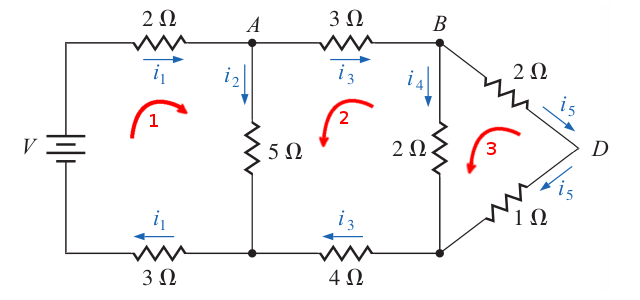
\includegraphics[height=4cm]{circuito1.png}}
                    \column{0.3\textwidth}                
                        {$ \left\{ \begin{array}{r}
                        5 i_1 + 5 i_2 = 5.5\\
                        5 i_2 - 7 i_3 - 2 i_4 = 0\\
                        2 i_4 - 3 i_5 = 0\\
                        i_1 = i_2 + i_3\\
                        i_3 = i_4 + i_5
                        \end{array} \right\}$}
                \end{columns} \\ \ \\ \ \\
                $\left( \begin{array}{ccccc}
                5 & 5 & 0 & 0 & 0\\
                0 & 5 & - 7 & - 2 & 0\\
                0 & 0 & 0 & 2 & - 3\\
                1 & - 1 & - 1 & 0 & 0\\
                0 & 0 & 1 & - 1 & - 1
                \end{array} \right) \cdot \left( \begin{array}{c}
                i_1\\  i_2\\  i_3\\  i_4\\  i_5
                \end{array} \right) = \left( \begin{array}{c}
                5.5\\  0\\  0\\  0\\  0
                \end{array} \right) \rightarrow \left\{ \begin{array}{l}
                i_1 = 0.6785\\
                i_2 = 0.4215\\
                i_3 = 0.2570\\
                i_4 = 0.1542\\
                i_5 = 0.1028
                \end{array} \right\}$
            \end{exampleblock}
        \end{frame}
        \begin{frame}{Cálculo de circuito eléctrico}
            \begin{exampleblock}{Mallas}
                \begin{center}
                    {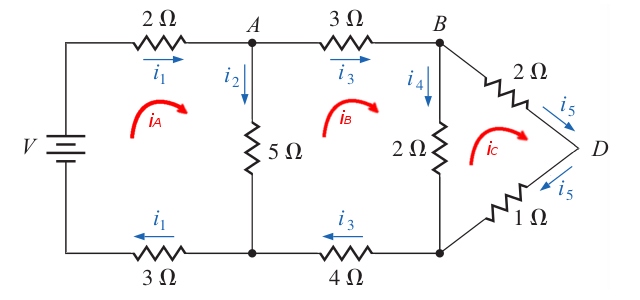
\includegraphics[height=5cm]{circuito2.png}}
                \end{center}
                {$\left( \[\arraycolsep=4pt\def\arraystretch{1} \begin{array}{ccc}
                10 & - 5 & 0\\
                - 5 & 14 & - 2\\
                0 & - 2 & 5 
                \end{array} \right) \cdot \left( \[\arraycolsep=1pt\def\arraystretch{1} \begin{array}{c}
                i_A\\  i_B\\  i_C
                \end{array} \right) = \left( \begin{array}{c}
                5.5\\  0\\  0
                \end{array} \right) \rightarrow \left\{ \begin{array}{l}
                i_A = 0.6785\\
                i_B = 0.2570\\
                i_C = 0.1028
                \end{array} \right\} \rightarrow \left\{ \begin{array}{l}
                i_1 = i_A = 0.6785\\
                i_2 = i_A - i_B = 0.4215\\
                i_3 = i_B = 0.2570\\
                i_4 = i_B - i_C = 0.1542\\
                i_5 = i_C = 0.1028
                \end{array} \right\}$}
            \end{exampleblock}
        \end{frame}
    \subsection{Circuito hidráulico}
        \begin{frame}{Cálculo de circuito hidráulico}
            \begin{exampleblock}{Cálculo de presiones en nudos de circuito hidráulico cerrado}
            \begin{center}
                {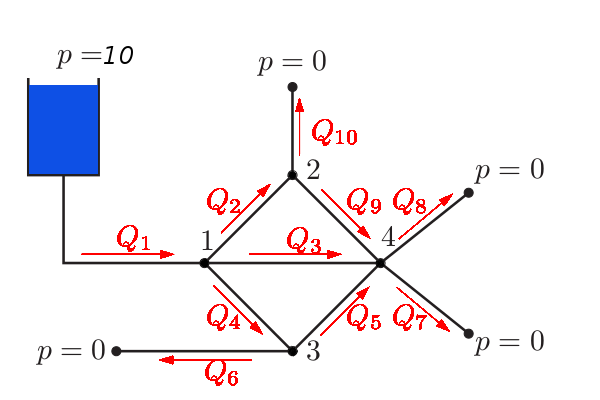
\includegraphics[height=5cm]{hidraulic.png}}
            \end{center} \\ \ \\ 
            {$\left. \begin{array}{ll}
            Nudo \ 1 : & Q_1 = Q_2 + Q_3 + Q_4\\
            Nudo \ 2 : & Q_2 = Q_{10} + Q_9\\
            Nudo \ 3 : & Q_4 = Q_5 + Q_6\\
            Nudo \ 4 : & Q_9 + Q_3 + Q_5 = Q_8 + Q_7
            \end{array} \right\}$} \ \ \  \ \ \ \ \ \ \ \ \ \ \ \ \ \ \Large{$Q_j = k L\tmmathbf{\Delta}p_j $}
            \end{exampleblock}
        \end{frame}
        \begin{frame}{Cálculo de circuito hidráulico}
            \begin{exampleblock}{Cálculo de presiones en nudos de circuito hidráulico cerrado (y II)}
                \begin{center}
                    {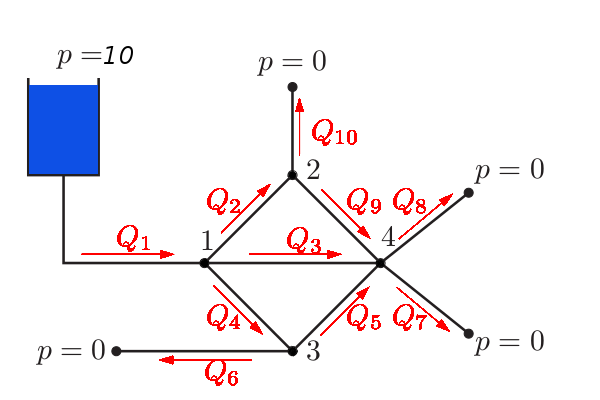
\includegraphics[height=3cm]{hidraulic.png}} \\ \ \\
                    {$\begin{array}{|l|c|r|}
                    \hline
                    \tmop{tuberia} & k & L\\
                    \hline
                    1 & 0.01 & 20\\
                    \hline
                    2 & 0.005 & 10\\
                    \hline  
                    3 & 0.005 & 14\\
                    \hline
                    4 & 0.005 & 10\\
                    \hline
                    5 & 0.005 & 10\\
                    \hline
                    6 & 0.002 & 8\\
                    \hline
                    7 & 0.002 & 8\\
                    \hline
                    8 & 0.002 & 8\\
                    \hline
                    9 & 0.005 & 10\\
                    \hline
                    10 & 0.002 & 8\\
                    \hline
                    \end{array} \rightarrow Q_j = k L\tmmathbf{\Delta}p_j \rightarrow \left\{ \begin{array}{l}
                    Q_1 = 0.2 ( 10 - P_1)\\
                    Q_2 = 0.05 ( P_1 - P_2)\\
                    Q_3 = 0.07 ( P_1 - P_4)\\
                    Q_4 = 0.05 ( P_1 - P_3)\\   
                    Q_5 = 0.05 ( P_3 - P_4)\\       
                    Q_6 = 0.016 ( P_3)\\    
                    Q_7 = 0.016 ( P_4)\\
                    Q_8 = 0.016 ( P_4)\\
                    Q_9 = 0.05 ( P_2 - P_4)\\
                    Q_{10} = 0.016 ( P_2)
                    \end{array}$}
                \end{center}
            \end{exampleblock}
        \end{frame}
        \begin{frame}{Cálculo de circuito hidráulico}
            \begin{exampleblock}{Cálculo de presiones en nudos de circuito hidráulico cerrado (y III)}
                \begin{center}
                    {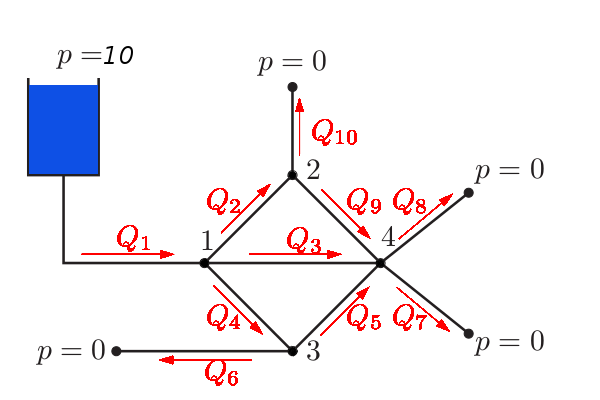
\includegraphics[height=3.5cm]{hidraulic.png}} \\ \ \\
                    {$\left\{ \begin{array}{l}
                    0.2 ( 10 - P_1) = 0.05 ( P_1 - P_2) + 0.07 ( P_1 - P_4) + 0.05 ( P_1 - P_3)\\
                    0.05 ( P_1 - P_2) = 0.05 ( P_2 - P_4) + 0.016 ( P_2)\\
                    0.05 ( P_1 - P_3) = 0.05 ( P_3 - P_4) + 0.016 ( P_3)\\
                    0.05 ( P_2 - P_4) + 0.07 ( P_1 - P_4) + 0.05 ( P_3 - P_4) = 0.016 ( P_4) + 0.016 ( P_4)
                    \end{array} \right\} \rightarrow \\ \ \\ \ \\  \rightarrow \left\{ \begin{array}{l}
                    2 - 0.2 P_1 = 0.05 P_1 - 0.05 P_2 + 0.07 P_1 - 0.07 P_4 + 0.05 P_1 - 0.05 P_3\\
                    0.05 P_1 - 0.05 P_2 = 0.05 P_2 - 0.05 P_4 + 0.016 P_2\\
                    0.05 P_1 - 0.05 P_3 = 0.05 P_3 - 0.05 P_4 + 0.016 P_3\\
                    0.05 P_2 - 0.05 P_4 + 0.07 P_1 - 0.07 P_4 + 0.05 P_3 - 0.05 P_4 = 2 \cdot 0.016 P_4
                    \end{array} \right\} \rightarrow$}
                \end{center}
            \end{exampleblock}
        \end{frame}
        \begin{frame}{Cálculo de circuito hidráulico}
            \begin{exampleblock}{Cálculo de presiones en nudos de circuito hidráulico cerrado (y IV)}
                \begin{center}
                    {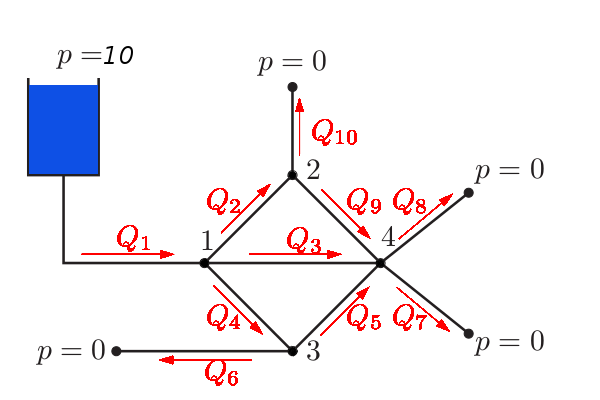
\includegraphics[height=3.5cm]{hidraulic.png}} \\ \ \\
                    {$\left\{ \begin{array}{r}
                    - 0.37 P_1 + 0.05 P_2 + 0.05 P_3 + 0.07 P_4 = - 2\\
                    0.05 P_1 - 0.016 P_2 + 0.05 P_4 = 0\\
                    0.05 P_1 - 0.116 P_3 + 0.05 P_4 = 0_{}\\
                    0.07 P_1 + 0.05 P_2 + 0.05 P_3 - 0.202 P_4 = 0
                    \end{array} \right\} \\ \ \\ \ \\ \left( \begin{array}{cccc}
                    - 0.37 & 0.05 & 0.05 & 0.07\\
                    0.05 & - 0.016 & 0 & 0.05\\
                    0.05 & 0 & - 0.116 & 0.05\\
                    0.07 & 0.05 & 0.05 & - 0.202
                    \end{array} \right) \left( \begin{array}{l}
                    P_1\\  P_2\\  P_3\\  P_4
                    \end{array} \right) = \left( \begin{array}{c}
                    - 2\\  0\\  0\\  0
                    \end{array} \right) \rightarrow \left\{ \begin{array}{l}
                    P_1 = 8.1172 \tmop{bar}\\
                    P_2 = 5.9893 \tmop{bar}\\
                    P_3 = 5.9893 \tmop{bar}\\
                    P_4 = 5.7779 \tmop{bar}
                    \end{array} \right.$}
                \end{center}
            \end{exampleblock}
        \end{frame}
\section{Conclusiones}
    \subsection{}
        \begin{frame}{¿Directo o iterado? - Matriz llena}
            \begin{center}
                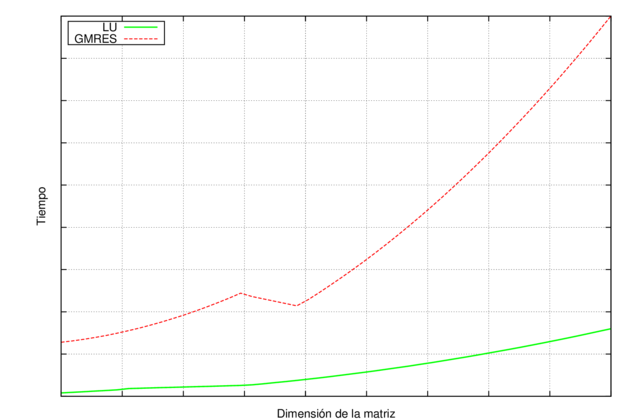
\includegraphics[height=7cm]{m_llena.png}
            \end{center}
        \end{frame}
        \begin{frame}{¿Directo o iterado? - Matriz de banda estrecha}
            \begin{center}
                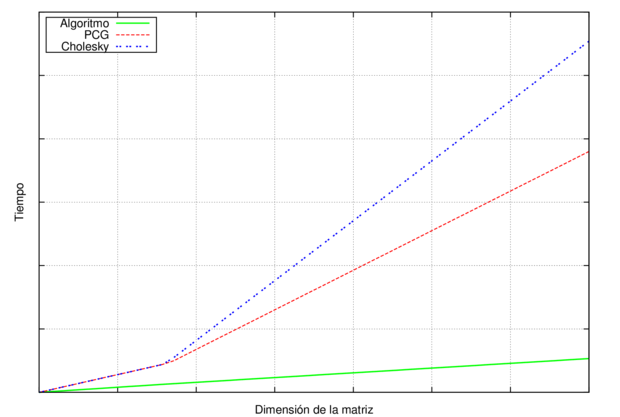
\includegraphics[height=7cm]{m-simetricaestrecha.png}
            \end{center}
        \end{frame}
        \begin{frame}{¿Directo o iterado? - Matriz de banda ancha}
            \begin{center}
                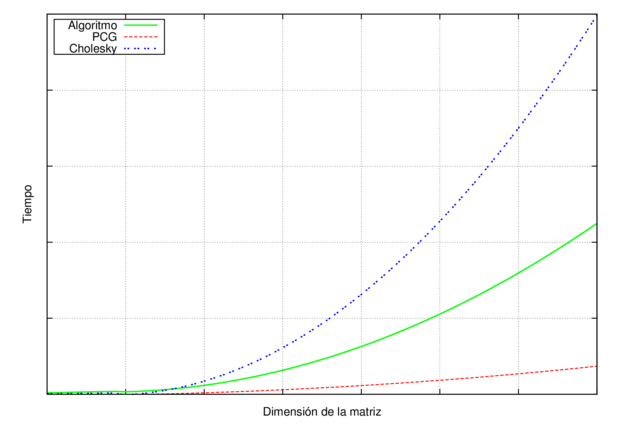
\includegraphics[height=7cm]{m-simetricaancha.png}
            \end{center}
        \end{frame}
    \subsection{Recursos utilizados}
        \begin{frame}{Recursos Utilizados}
            \begin{block}{Python}
                \begin{itemize}
                    \item Python tiene una sintaxis clara
                    \item Python es de propósito general
                    \item Python es dinámico
                    \item Python es amigo de C/C++ y Fortran
                    \item Python es libre 
                \end{itemize}
                \begin{center}
                    
\includegraphics[height=4.8cm]{pythoneco.png}
                \end{center}
            \end{block}
        \end{frame}
        \begin{frame}{Recursos Utilizados}
            \begin{block}{Cómo comenzar en Python}
                \begin{itemize}
                    \item Tutorial oficial: \\ \url {http://docs.python.org.ar/tutorial/2/contenido.html}
                    \item Pybonacci: blog de Python científico
                    \item Aeropython: \\ \url {https://github.com/AeroPython/Curso_AeroPython}
                    \item Python para ingenieros: \\ \url {http://cacheme.org/curso-online-python-cientifico-ingenieros/}
                    \item Lorena Barba: profesora el GWU    
                    \item Numerical MOOC: \\  \url {http://openedx.seas.gwu.edu/courses/GW/MAE6286/2014_fall/about}
                    \item Stack Overflow: \\ \url {http://stackoverflow.com/}
                \end{itemize}
            \end{block}
        \end{frame}
        \begin{frame}{Recursos Utilizados}
            \begin{center}
                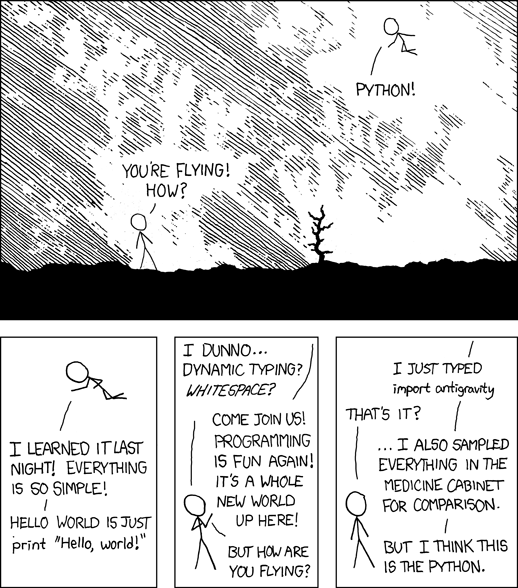
\includegraphics[height=7.5cm]{pythonjoke.png}
            \end{center}
        \end{frame}
        \begin{frame}{Recursos Utilizados}
            \begin{block}{\LaTeX{}}
                Ventajas: \\
                    \begin{itemize}
                        \item {Es estable y multiplataforma} 
                        \item {Alta calidad en la edición de ecuaciones}
                        \item {Facilita la creación de documentos estructurados} 
                        \item {Es gratis}
                    \end{itemize}\\ \ \\ 
                Inconvenientes: \\
                    \begin{itemize}
                        \item {Dificultad avanzada y curva de aprendizaje lenta} 
                        \item {No se ven los resultados hasta que se compila el archivo} 
                    \end{itemize}\\ 
                \begin{center}
                    
\includegraphics[height=3cm]{latex.png}
                \end{center}
            \end{block}
        \end{frame}
        \begin{frame}{Recursos Utilizados}
            \begin{block}{Cómo comenzar en \LaTeX{}}
                \begin{itemize}
                    \item<1-> TeXmacs $\rightarrow$ LyX \\
                    \item<2-> TeXStudio / TeXLive
                    \item<3-> ShareLatex \\ \url{https://es.sharelatex.com}
                    \item<4-> Pagina TeX español... \\ \url {http://www.cervantex.es}
                    \item<5-> ...y lo que mas útil es, su sección de FAQ \\ \url {http://www.aq.upm.es/Departamentos/Fisica/agmartin/webpublico/latex/FAQ-CervanTeX/FAQ-CervanTeX.html}
                    \item<6-> Videotutoriales en castellano: \\ \url {https://es.sharelatex.com/blog/latex-guides/beginners-tutorial.html}
                    \item<7-> Tutorial desde cero: \\ \url{http://mate.dm.uba.ar/~pdenapo/tutorial-latex/tutorial-latex.html}
                    \item<8-> Stack Overflow: \\ \url {http://stackoverflow.com/}
                \end{itemize}
            \end{block}
        \end{frame}

\begin{frame}{Bibliografía}
    \begin{itemize}
        \item BURDEN, R; FAIRES, J; 2010. Numerical Analysis; Cengage Learning
        \item MOIN, P; 2010. Fundamentals of engineering - Numerical Analysis; Cambridge
        \item QUARTERONI, A; SALERI, F; 2006. Cálculo matemático con MATLAB y Octave; Springer
        \item FANGOHR, H; 2014. Python for computational science and engineering; Southampton
    \end{itemize}
\end{frame}

\end{document}